\documentclass[toc=chapterentrywithdots]{scrbook}
\usepackage[brazil]{babel}
\usepackage[T1]{fontenc}
\usepackage{multicol}
%\usepackage{scrlayer-scrpage}
\usepackage{verbatim}
\usepackage{graphicx}
\usepackage[export]{adjustbox}
\usepackage{listings}
\lstset{
  basicstyle=\ttfamily
}
% \automark[chapter]{chapter}
% \clearpairofpagestyles
% \ohead{\pagemark}
% \ihead{\headmark}
\clubpenalty=10000 
\widowpenalty=10000
\displaywidowpenalty=10000
%\chead{\footnotesize\headmark}
% \cfoot{\footnotesize\pagemark}
\setlength{\parskip}{3.5pt}
%
\makeatletter
\setlength{\@fptop}{0pt}
\makeatother
\setlength{\parindent}{20pt}

\NewDocumentCommand{\cmd}{m}{\texttt{\symbol{`\\}#1}} %permite colocar comandos dentro de comandos ou no texto.


\begin{document}
\frontmatter
\title{Breves Anotações sobre \KOMAScript}
\author{Baena}
\date{\today}
\maketitle
\tableofcontents
\frontmatter
\chapter{Introdução}
Este capítulo contém, entre outras coisas, informações importantes sobre a estrutura do manual e a história do \KOMAScript\, que começa anos antes da primeira versão. Você também encontrará informações sobre como instalar o \KOMAScript\ e o que fazer se encontrar erros.

\section{Nota preliminar}
O \KOMAScript\ é muito complexo. Isso se deve ao fato de que ele consiste não apenas em uma única classe ou um único pacote, mas em um conjunto de muitas classes e pacotes. Embora as classes sejam projetadas como contrapartes das classes padrão, isso não significa que elas forneçam apenas os comandos, ambientes e configurações das classes padrão, ou que imitem sua aparência. Os recursos do \KOMAScript\ às vezes superam em muito os das classes padrão. Alguns deles devem ser considerados extensões dos recursos básicos do kernel \LaTeX.

O exposto acima significa que a documentação do \KOMAScript\ deve ser extensa. Além disso, o \KOMAScript\ normalmente não é ensinado. Isso significa que não há professores que conheçam seus alunos e possam, portanto, escolher os materiais didáticos e adaptá-los adequadamente. Seria fácil escrever documentação para um público específico. A dificuldade enfrentada pelo autor, no entanto, é que o manual deve atender a todos os públicos potenciais. Tentei criar um guia que seja igualmente adequado para o cientista da computação e a secretária do peixeiro. Eu tentei, embora esta seja realmente uma tarefa impossível. O resultado são vários compromissos, e eu pediria que você levasse esse problema em consideração se tiver alguma reclamação ou sugestão para ajudar a melhorar a situação atual.

Apesar da extensão deste manual, eu pediria que você consultasse a documentação primeiro caso tenha problemas. Você deve começar consultando o índice de várias partes no final deste documento. Além deste manual, a documentação inclui todos os documentos de texto que fazem parte do pacote. Veja manifest.tex para uma lista completa.
\section{Estrutura do Guia}
Este manual é dividido em várias partes: Há uma seção para usuários comuns, uma para usuários avançados e especialistas, e um apêndice com mais informações e exemplos para aqueles que querem entender o \KOMAScript\ completamente.

A Parte I é destinada a todos os usuários do \KOMAScript. Isso significa que algumas informações nesta seção são direcionadas a novatos no \LaTeX. Em particular, esta parte contém muitos exemplos que visam esclarecer as explicações. Não hesite em experimentar esses exemplos você mesmo e descobrir como o \KOMAScript\ funciona modificando-os. Dito isso, o guia do usuário do \KOMAScript\ não pretende ser uma cartilha do \LaTeX. Aqueles que são novos no \LaTeX devem dar uma olhada em The Not So Short Introduction ao \LaTeXe ou \LaTeXe para Autores ou um livro de referência \LaTeX. Você também encontrará informações úteis nas muitas FAQs do \LaTeX, incluindo as Perguntas Frequentes do \TeX\ na Web. Embora o tamanho das Perguntas Frequentes do \TeX\ na Web seja considerável, você deve obter pelo menos uma visão geral aproximada e consultá-la caso tenha problemas, bem como este guia.

A Parte II é destinada a usuários avançados do \KOMAScript\, aqueles que já estão familiarizados com \LaTeX\ ou que trabalham com o \KOMAScript\ há algum tempo e querem entender mais sobre como ele funciona, como ele interage com outros pacotes e como executar tarefas mais especializadas com ele. Para esse propósito, retornamos a alguns aspectos das descrições de classe da Parte I e os explicamos em mais detalhes. Além disso, documentamos alguns comandos que são particularmente destinados a usuários avançados e especialistas. Isto é complementado pela documentação de pacotes que normalmente são escondidos do usuário, na medida em que eles fazem seu trabalho abaixo da superfície das classes e pacotes do usuário. Esses pacotes são especificamente projetados para serem usados por autores de classes e pacotes.

O apêndice, que só pode ser encontrado na versão do livro em alemão, contém informações além daquelas que são cobertas na parte I e parte II. Usuários avançados encontrarão informações básicas sobre questões de tipografia para dar a eles uma base para suas próprias decisões. Além disso, o apêndice fornece exemplos para aspirantes a autores de pacotes. Esses exemplos não se destinam simplesmente a serem copiados. Em vez disso, eles fornecem informações sobre planejamento e implementação de projetos, bem como alguns comandos básicos do \LaTeX\ para autores de pacotes.

O layout do guia deve ajudá-lo a ler apenas as partes que são realmente de interesse. Cada classe e pacote normalmente tem seu próprio capítulo. Referências cruzadas para outro capítulo são, portanto, geralmente também referências a outra parte do pacote geral. No entanto, como as três principais classes (scrbook, scrrprt e scrartcl) concordam amplamente, elas são apresentadas juntas no capítulo 3. Diferenças entre as classes, por exemplo, para algo que afeta apenas a classe scrartcl, são claramente destacadas na margem, como mostrado aqui com scrartcl.

A documentação primária do \KOMAScript\ está em alemão e foi traduzida para sua conveniência; como a maioria do mundo \LaTeX, seus comandos, ambientes, opções, etc., estão em inglês. Em alguns casos, o nome de um comando pode soar um pouco estranho, mas mesmo assim, esperamos e acreditamos que com a ajuda deste guia, o \KOMAScript\ será utilizável e útil para você.

Neste ponto, você deve saber o suficiente para entender o guia. No entanto, ainda pode valer a pena ler o restante deste capítulo.

\section{História do \KOMAScript}
No início dos anos 1990, Frank Neukam precisava de um método para publicar as notas de aula de um instrutor. Naquela época, o \LaTeX\ era \LaTeXe\ e não havia distinção entre classes e pacotes — havia apenas estilos. Frank sentiu que os estilos de documentos padrão não eram bons o suficiente para seu trabalho; ele queria comandos e ambientes adicionais. Ao mesmo tempo, ele estava interessado em tipografia e, depois de ler\textit{ Ausgewählte Aufsätze über Fragen der Gestalt des Buches und der Typographie}, de Tschichold (Artigos selecionados sobre os problemas de design de livros e Tipografia), ele decidiu escrever seu próprio estilo de documento — e não apenas uma solução única para suas notas de aula, mas uma família de estilos inteira, uma projetada especificamente para tipografia europeia e alemã. Assim nasceu o Script.

Markus Kohm, o desenvolvedor do \KOMAScript\, encontrou o Script em dezembro de 1992 e adicionou uma opção para usar o formato de papel A5. Naquela época, nem o estilo padrão nem o Script forneciam suporte para papel A5. Portanto, não demorou muito para que Markus fizesse as primeiras alterações no Script. Essas e outras alterações foram então incorporadas ao Script-2, lançado por Frank em dezembro de 1993.

Em meados de 1994, o \LaTeXe\ ficou disponível e trouxe consigo muitas alterações. Usuários do Script-2 enfrentaram a opção de limitar seu uso ao modo de compatibilidade do \LaTeXe\ ou desistir do Script completamente. Essa situação levou Markus a montar um novo pacote \LaTeX2e, lançado em 7 de julho de 1994 como \KOMAScript\. Poucos meses depois, Frank declarou o \KOMAScript\ como o sucessor oficial do Script. O \KOMAScript\ originalmente não fornecia nenhuma classe \textit{letter}, mas essa deficiência foi logo corrigida por Axel Kielhorn, e o resultado se tornou parte do \KOMAScript\ em dezembro de 1994. Axel também escreveu o primeiro verdadeiro guia do usuário em alemão, que foi seguido por um guia em inglês de Werner Lemberg.

Desde então, muito tempo se passou. O\ LaTeX\ mudou apenas em pequenas coisas, mas o seu cenário mudou muito; muitos novos pacotes e classes estão agora disponíveis e o próprio \KOMAScript\ cresceu muito além do que era em 1994. O objetivo inicial era fornecer boas classes LaTeX para autores de língua alemã, mas hoje seu propósito principal é fornecer alternativas mais flexíveis às classes padrão. O sucesso do \KOMAScript\ levou a e-mails de usuários de todo o mundo, e isso levou a muitas novas macros — todas precisando de documentação; daí este “pequeno guia”.

\section{Agradecimentos especiais}
Agradecimentos na introdução? Não, os agradecimentos adequados podem ser encontrados no adendo. Meus comentários aqui não são destinados aos autores deste guia — e esses agradecimentos devem vir de você, o leitor, de qualquer forma. Eu, o autor do \KOMAScript, gostaria de estender meus agradecimentos pessoais a Frank Neukam. Sem sua família Script, \KOMAScript\ não teria surgido. Sou grato às muitas pessoas que contribuíram para o \KOMAScript\, mas com sua indulgência, gostaria de mencionar especificamente Jens-Uwe Morawski e Torsten Krüger. A tradução em inglês do guia é, entre muitas outras coisas, devido ao comprometimento incansável de Jens. Torsten foi o melhor testador beta que já tive. Seu trabalho melhorou particularmente a usabilidade do scrlttr2 e scrpage2. Muito obrigado a todos que me encorajaram a continuar, a tornar as coisas melhores e menos propensas a erros, ou a implementar recursos adicionais.

Agradecimentos especiais também aos fundadores e membros do DANTE, Deutschsprachige Anwendervereinigung \TeX\ e.V, (Grupo de Usuários do \TeX\ em Língua Alemã). Sem o servidor DANTE, o \KOMAScript\ não poderia ter sido lançado e distribuído. Obrigado também a todos nos grupos de notícias e listas de discussão do \TeX\ que respondem perguntas e me ajudaram a dar suporte ao \KOMAScript.

Meus agradecimentos também vão para todos aqueles que sempre me encorajaram a ir além e implementar este ou aquele recurso melhor, com menos falhas, ou simplesmente como uma extensão. Eu também gostaria de agradecer ao doador muito generoso que me deu a quantia mais significativa de dinheiro que eu já recebi pelo trabalho feito até agora no \KOMAScript.

\mainmatter
\chapter{\KOMAScript\ para Autores}
Esta parte fornece informações para escritores de artigos, relatórios, livros e cartas. O usuário médio provavelmente está menos interessado em como as coisas são implementadas no \KOMAScript\ e quais armadilhas existem. Além disso, usuários normais não estão interessados em opções e instruções obsoletas. Eles querem saber como fazer as coisas usando opções e instruções atuais, e talvez em algumas informações básicas sobre tipografia.

As poucas passagens nesta parte que contêm informações e explicações extras que podem ser de menos interesse para o leitor impaciente são definidas em uma fonte sans-serif e podem ser puladas se desejado. Para aqueles que estão interessados em mais informações sobre a implementação, efeitos colaterais com outros pacotes ou opções e instruções obsoletas, consulte a parte II começando na página 335. Essa parte do guia \KOMAScript\ também descreve todos os recursos que foram criados especialmente para autores de pacotes e classes.
\chapter{Calculando o Layout da Página com typearea}
Muitas classes \LaTeX, incluindo as classes padrão, apresentam ao usuário uma configuração amplamente fixa de margens e layout de página. Nas classes padrão, a escolha é limitada a selecionar um tamanho de fonte. Existem pacotes separados, como geometry, que dão ao usuário controle completo sobre, mas também total responsabilidade por, definir a área de tipo e margens.

O \KOMAScript\ adota uma abordagem um pouco diferente com o pacote typearea. Os usuários recebem maneiras de ajustar o design e os algoritmos com base em padrões tipográficos estabelecidos, tornando mais fácil para eles fazerem boas escolhas.

No LaTeX, o espaçamento entre linhas é definido em cerca de 20\% do tamanho da fonte.
Comprimentos de linha acima de 80 caracteres são inaceitáveis.

O \LaTeX\ reconhece os comandos \verb|\raggedbottom| e \verb|\flushbottom|. \verb|\raggedbottom| especifica que a última linha de uma página deve ser posicionada onde quer que tenha sido calculada. Isso significa que a posição desta linha pode ser diferente em cada página, até a altura de uma linha — ainda mais quando o fim da página coincide com títulos, figuras, tabelas ou similares. Em documentos frente e verso isso geralmente é indesejável. O segundo comando, \verb|\flushbottom|, garante que a última linha esteja sempre na borda inferior da área de texto. Para obter essa compensação vertical, o  \LaTeX\ pode ter que esticar a cola vertical além do que é normalmente permitido. O salto de parágrafo é uma cola vertical tão elástica, mesmo quando definido como zero. Para evitar esticar em páginas normais onde o espaçamento de parágrafo é a única cola elástica, a altura da área de texto deve ser um múltiplo da altura da linha de texto, incluindo a distância da primeira linha do topo da área de texto.

\section{Construindo a Área de Tipo por Divisão}
A maneira mais fácil de garantir que a área de texto tenha a mesma proporção da página é a seguinte:

 \begin{enumerate}
     \item Primeiro, subtraia o BCOR necessário para a correção de encadernação da borda interna do papel e divida o restante da página verticalmente em linhas DIV de altura igual.
     \item Em seguida, divida a página horizontalmente no mesmo número (DIV) de colunas de largura igual.
     \item Pegue a linha mais alta como a margem superior e as duas linhas mais baixas como a margem inferior. Se estiver imprimindo frente e verso, você também pega a coluna mais interna como a margem interna e as duas colunas mais externas como a margem externa.
     \item Adicione o BCOR de correção de encadernação à margem interna.
 \end{enumerate}
\bigskip
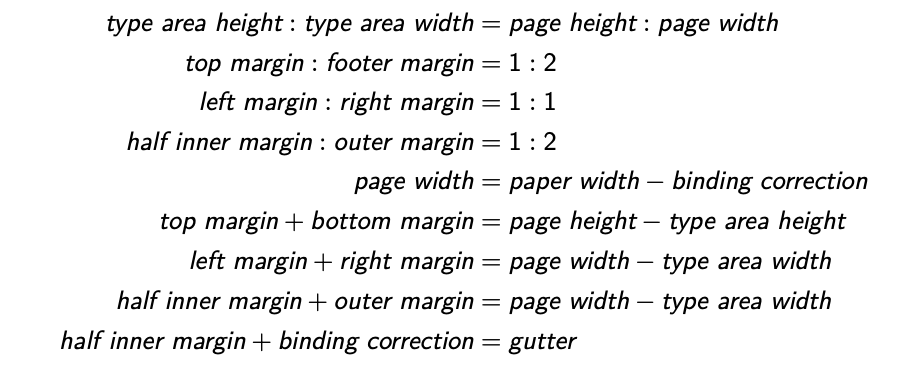
\includegraphics[scale=0.8]{imagem01.png}

\chapter{Fundamentos do Layout de Página}
À primeira vista, uma única página de um livro ou outro material impresso consiste em margens, um cabeçalho, um corpo de texto e um rodapé. Mais precisamente, há também um espaço entre a área do cabeçalho e o corpo do texto, bem como entre o corpo e o rodapé. O corpo do texto é chamado, no jargão de tipógrafos e compositores, de área de tipo. A divisão dessas áreas, bem como suas relações entre si e com o papel, é chamada de layout de página.

Vários algoritmos e métodos heurísticos para construir uma área de tipo apropriada foram discutidos na literatura. Essas regras são conhecidas como os “cânones da construção de páginas”. Uma abordagem frequentemente mencionada envolve diagonais e suas interseções. O resultado é que a proporção da área de tipo corresponde às proporções da página. Em um documento de um lado, as margens esquerda e direita devem ter larguras iguais, enquanto a proporção das margens superior e inferior deve ser 1:2. Em um documento frente e verso (por exemplo, um livro), no entanto, toda a margem interna (a margem na lombada) deve ter o mesmo tamanho que cada uma das duas margens externas; em outras palavras, uma única página contribui com apenas metade da margem interna.

No parágrafo anterior, mencionamos e enfatizamos a página. Muitas vezes, pensa-se erroneamente que o formato da página é o mesmo que o formato do papel. No entanto, se você olhar para um documento encadernado, poderá ver que parte do papel desaparece na encadernação e não faz mais parte da página visível. Para a área do tipo, no entanto, não é o formato do papel que é importante; é a impressão da página visível para o leitor. Assim, fica claro que o cálculo da área do tipo deve levar em conta o papel “perdido” na encadernação e adicionar essa quantidade à largura da margem interna. Isso é chamado de correção de encadernação. A correção de encadernação é, portanto, calculada como parte da medianiz, mas não da margem interna visível.

A correção de encadernação depende do processo de produção e não pode ser definida em termos gerais. Portanto, é um parâmetro que deve ser redefinido para cada projeto. Na impressão profissional, esse valor desempenha apenas um papel menor, pois a impressão é feita em folhas maiores de papel e depois cortada no tamanho certo. O corte é feito para que as relações acima para a página visível, frente e verso sejam mantidas.

\section*{Layout de dois lados com a construção de caixa da divisão clássica de nove partes, após subtrair uma correção de encadernação:
}
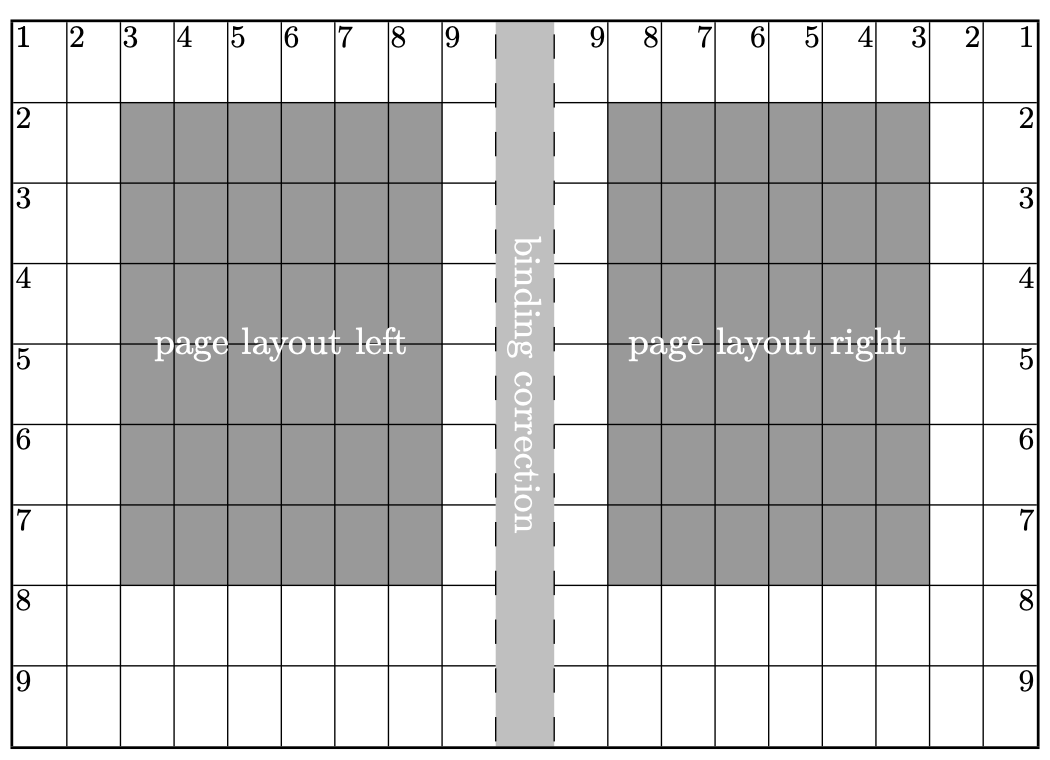
\includegraphics[scale=0.8]{imagem02.png}

O que resta na página é a área de texto. A largura e a altura da área de texto e margens resultam automaticamente do número de linhas e colunas, DIV. Como as margens sempre precisam de três listras, DIV deve ser maior que três. Para que a área de texto ocupe pelo menos o dobro de espaço das margens, DIV deve ser pelo menos nove. Com esse valor, o design também é conhecido como a divisão clássica de nove partes.

No \KOMAScript\ esse tipo de design é implementado com o pacote typearea, onde a margem inferior pode remover quaisquer frações de uma linha para cumprir com a restrição para a altura da área de tipo mencionada no parágrafo anterior e, assim, reduzir o problema mencionado com \verb|\flushbottom|. Para papel A4, DIV é predefinido de acordo com o tamanho da fonte (veja tabela 2.2, página 36). Se não houver correção de encadernação (BCOR = 0 pt), os resultados correspondem aproximadamente aos valores da tabela 2.1, página 35.

Além dos valores predefinidos, você pode especificar BCOR e DIV como opções ao carregar o pacote (veja a seção 2.4, começando na página 33). Há também um comando para calcular a área do tipo explicitamente fornecendo esses valores como parâmetros (veja também a seção 2.4, página 39).

\begin{verbatim}
            \typearea[BCOR]{DIV}
            \recalctypearea
\end{verbatim}


O pacote typearea pode determinar automaticamente o valor ideal de DIV para a fonte e entrelinhamento usados.

\section{Dimensões da área de tipo dependentes de DIV para A4 independentemente de \texttt{\char`\\topskip} ou BCOR}


\begin{figure}[h]
    \centering
    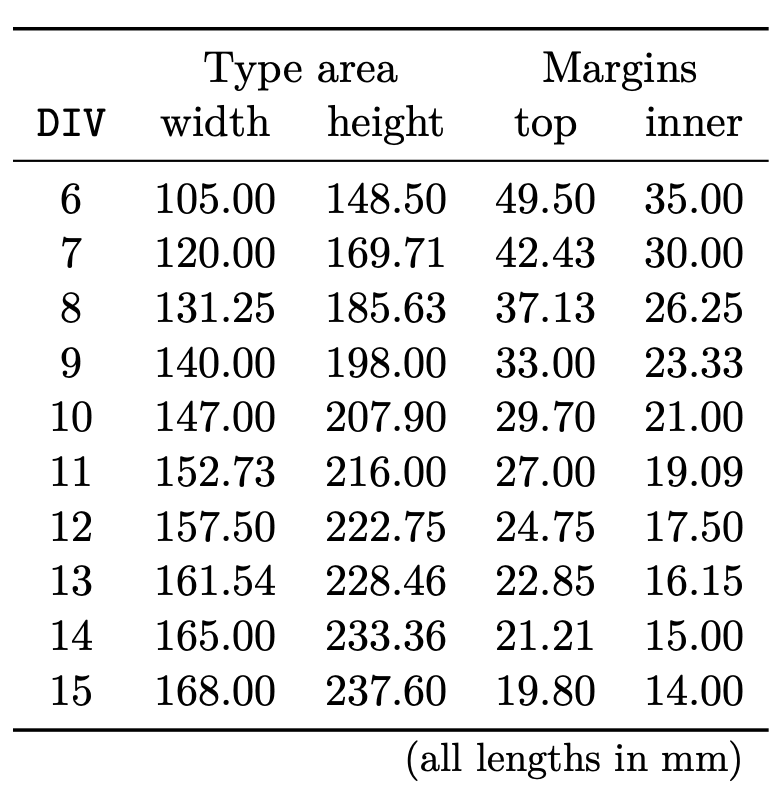
\includegraphics[width=0.55\linewidth]{tab2_1.png}
    \caption{Tabela 2.1 do Manual}
    \label{fig:tab2_1l}
\end{figure}

\section{DIV defaults for A4 in all \KOMAScript\ classes:}
\begin{figure}[h]
    \centering
    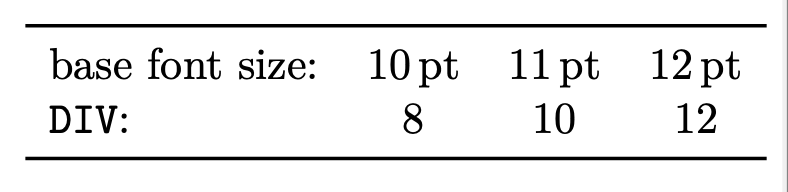
\includegraphics[width=0.6\linewidth]{tab2_2.png}
    \caption{Tabela 2.2 do Manual}
    \label{fig:tab2_2}
\end{figure}


\chapter{Ajustando a Área de Tipo e o Layout da Página}
O pacote typearea oferece duas interfaces de usuário diferentes para influenciar a construção da área de tipo. O método mais importante é especificar opções ao carregar o pacote. Para informações sobre como configurar opções com o \KOMAScript\ consulte a seção 2.4. Nesta seção, as classes usadas nos exemplos não são classes \KOMAScript\ existentes, mas hipotéticas. Este guia assume que, idealmente, uma classe apropriada esteja disponível para cada tarefa.

\minisec{BCOR = correction}
Use a opção BCOR=correction para especificar o valor absoluto da correção de encadernação, ou seja, a largura da área perdida do papel durante o processo de encadernação. Este valor é então automaticamente levado em consideração ao construir o layout da página e é adicionado de volta à margem interna (ou esquerda) durante a saída. No valor da correção, você pode especificar qualquer unidade de medida entendida pelo TEX.

Ao usar uma classe \KOMAScript\ você não precisa carregar o pacote typearea explicitamente:
\begin{verbatim}
            \documentclass[BCOR=8.25mm]{scrreprt}
\end{verbatim}

Você pode omitir a opção a4paper com scrreprt, já que este é o padrão para todas as classes \KOMAScript.

Se você quiser definir a opção para um novo valor mais tarde, você pode, por exemplo, usar o seguinte:
\begin{verbatim}
            \documentclass{scrreprt}
            \KOMAoptions{BCOR=8.25mm}
\end{verbatim}

Os padrões são inicializados quando a classe scrreprt é carregada. Alterar uma configuração com os comandos \KOMAScript\ ou \verb|\KOMAoption| calculará automaticamente uma nova área de tipo com novas margens.
Note que você deve passar esta opção como uma opção de classe ao carregar uma das classes \KOMAScript\ como no exemplo acima, ou via \verb|\KOMAoptions| ou \verb|\KOMAoption| após carregar a classe. Quando você usa uma classe \KOMAScript\ você não deve carregar o pacote typearea explicitamente com \verb|\usepackage|, nem deve especificá-lo como um argumento opcional ao carregar o pacote se você estiver usando outra classe. Se a opção for alterada com \verb|\KOMAoptions| ou \verb|\KOMAoption| após carregar o pacote, a área de tipo e as margens são automaticamente recalculadas.

\minisec{DIV=factor}
A opção DIV=factor especifica o número de faixas nas quais a página é dividida horizontalmente e verticalmente durante a construção da área de texto. O método de construção exato é encontrado na seção 2.2. É importante perceber que quanto maior o fator, maior o bloco de texto e menores as margens. Qualquer valor inteiro maior que 4 é válido para fator.

Observe, no entanto, que valores grandes podem causar violações nas restrições nas margens da área de texto, dependendo de como você define outras opções. Em casos extremos, o cabeçalho pode cair fora da página. Ao usar a opção DIV=factor, você é responsável por cumprir com as restrições de margem e por escolher um comprimento de linha tipograficamente agradável.

Na tabela 2.1, você encontrará os tamanhos das áreas de texto para vários fatores DIV para a página A4 sem correção de encadernação. Nesse caso, as outras restrições que dependem do tamanho da fonte não são levadas em consideração.

Se for absolutamente necessário definir o texto com um espaçamento de linha de 1,5, não redefina \verb|\baselinestretch| em nenhuma circunstância. Embora esse procedimento seja recomendado com muita frequência, ele está obsoleto desde a introdução do \LaTeXe\ em 1994. No pior caso, use o comando \verb|\linespread|. Eu recomendo o pacote setspace, que não é parte do \KOMAScript. Você também deve deixar typearea recalcular uma nova área de tipo após alterar o espaçamento de linha. No entanto, você deve voltar ao espaçamento de linha normal para o título, e de preferência para o índice e várias listas — assim como a bibliografia e o índice. Para detalhes, veja a explicação de DIV=current.

Não raramente eu me pergunto por que eu me detenho em cálculos de typearea para um capítulo inteiro, quando seria muito mais fácil apenas fornecer um pacote com o qual você pode ajustar as margens como em um processador de texto. Muitas vezes é dito que tal pacote seria uma solução melhor em qualquer caso, já que todos sabem como escolher margens apropriadas, e que as margens calculadas pelo \KOMAScript\ não são tão boas assim. Eu gostaria de citar Hans Peter Willberg e Friedrich Forssmann, dois dos mais respeitados tipógrafos contemporâneos. (Você pode encontrar o original em alemão no guia alemão.):

\begin{quote}
 A prática de fazer as coisas por si mesmo é muito difundida, mas os resultados são frequentemente duvidosos porque tipógrafos amadores não veem o que está errado e não conseguem saber o que é importante. É assim que você se acostuma com tipografia incorreta e ruim. [\ldots] Agora, a objeção poderia ser feita de que tipografia é uma questão de gosto. Quando se trata de decoração, talvez se possa aceitar esse argumento, mas como tipografia é principalmente sobre informação, erros não só podem irritar, mas podem até mesmo causar danos.   
\end{quote}





\chapter[As principais classes]{As principais classes: scrbook, scrreprt e scrartcl}
\begin{figure}[h]
    \centering
    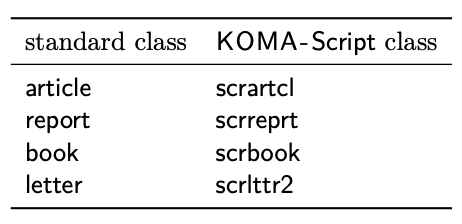
\includegraphics[width=0.60\linewidth]{classes.png}
    \caption{Principais Classes}
    \label{fig:class}
\end{figure}

Se você definir a opção dentro do documento, o tamanho da fonte principal e os tamanhos de fonte dependentes dos comandos \verb|\tiny|, \verb|\scriptsize|, \verb|\footnotesize|, \verb|\small|, \verb|\normalsize|, \verb|\large|, \verb|\Large|, \verb|\LARGE|, \verb|\huge| e \verb|\Huge| serão alterados. Isso pode ser útil, por exemplo, se você quiser que o apêndice seja definido em um tamanho de fonte menor.

Teoricamente, todas as declarações, incluindo texto literal, podem ser usadas como comandos. Você deve, no entanto, limitar-se àquelas declarações que realmente alteram apenas os atributos da fonte. Geralmente são comandos como \verb|\rmfamily|, \verb|\sffamily|, \verb|\ttfamily|, \verb|\upshape|, \verb|\itshape|, \verb|\slshape|, \verb|\scshape|, \verb|\mdseries|, \verb|\bfseries|, \verb|\normalfont|, bem como os comandos de tamanho de fonte \verb|\Huge|, \verb|\huge|, \verb|\LARGE|, \verb|\Large|, \verb|\large|, \verb|\normalsize|, \verb|\small|, \verb|\footnotesize|, \verb|\scriptsize| e \verb|\tiny|.


\chapter{Exemplo de código}
\textbf{Exemplo}: Suponha que você escreveu um livro de poesia e quer dedicá-lo ao seu cônjuge. Uma solução seria assim:
\begin{verbatim}
\documentclass{scrbook}
\usepackage[english]{babel}
\begin{document}
\extratitle{\textbf{\Huge In Love}}
\title{In Love}
\author{Prince Ironheart}
\date{1412}
\lowertitleback{This poem book was set with%
the help of {\KOMAScript} and {\LaTeX}}
\uppertitleback{Self-mockery Publishers}
\dedication{To my treasured hazel-hen\\
in eternal love\\
from your dormouse.}
\maketitle
\end{document} 
\end{verbatim}

Use seus nomes de animais de estimação favoritos para personalizá-lo.
\chapter[Table of Contents]{Table of Contents (Sumário/Índice)}

O título e o resumo opcional são normalmente seguidos por um índice. Frequentemente você também encontra listas adicionais de ambientes flutuantes, como tabelas e figuras, após o índice (veja a seção 3.20).

Além das opções documentadas nesta seção, os estilos do pacote tocbasic selecionados e configurados com
\verb|\DeclareTOCStyleEntry| (veja a página 387) também têm um impacto significativo na aparência do índice.

Similarmente, os comandos \char`\\\texttt{De\-cla\-re\-Sec\-tion\-Com\-mand}, \char`\\\texttt{Pro\-vi\-de\-Sec\-ti\-on\-Com\-mand}, \char`\\\texttt{Re\-de\-cla\-reSec\-ti\-onCom\-mand} documentados na seção 21.8, página 481 também podem afetar o índice.

O índice é normalmente formatado para que diferentes níveis de comandos de seccionamento tenham recuos diferentes. O número para cada nível é definido justificado à esquerda em um campo de largura fixa. Esta configuração padrão é selecionada com a opção \verb|toc=graduated|.

Se o nível de seccionamento que aparece no índice for muito profundo, o número para esse nível pode ser tão amplo que o espaço reservado para o número é insuficiente. O FAQ alemão [Wik] sugere redefinir o índice em tal caso. O \KOMAScript\ oferece um formato alternativo que evita o problema completamente. Se você usar a opção \verb|toc=flat|, nenhum recuo graduado será aplicado aos títulos dos níveis de seccionamento. Em vez disso, uma organização semelhante a uma tabela é usada, onde todos os números de seccionamento e títulos são definidos em uma coluna justificada à esquerda. O espaço necessário para os números de seção é, portanto, determinado automaticamente.

Você pode encontrar uma visão geral de todos os valores disponíveis para a configuração de \verb|toc| na tabela 3.5.

\begin{figure}
    \centering
    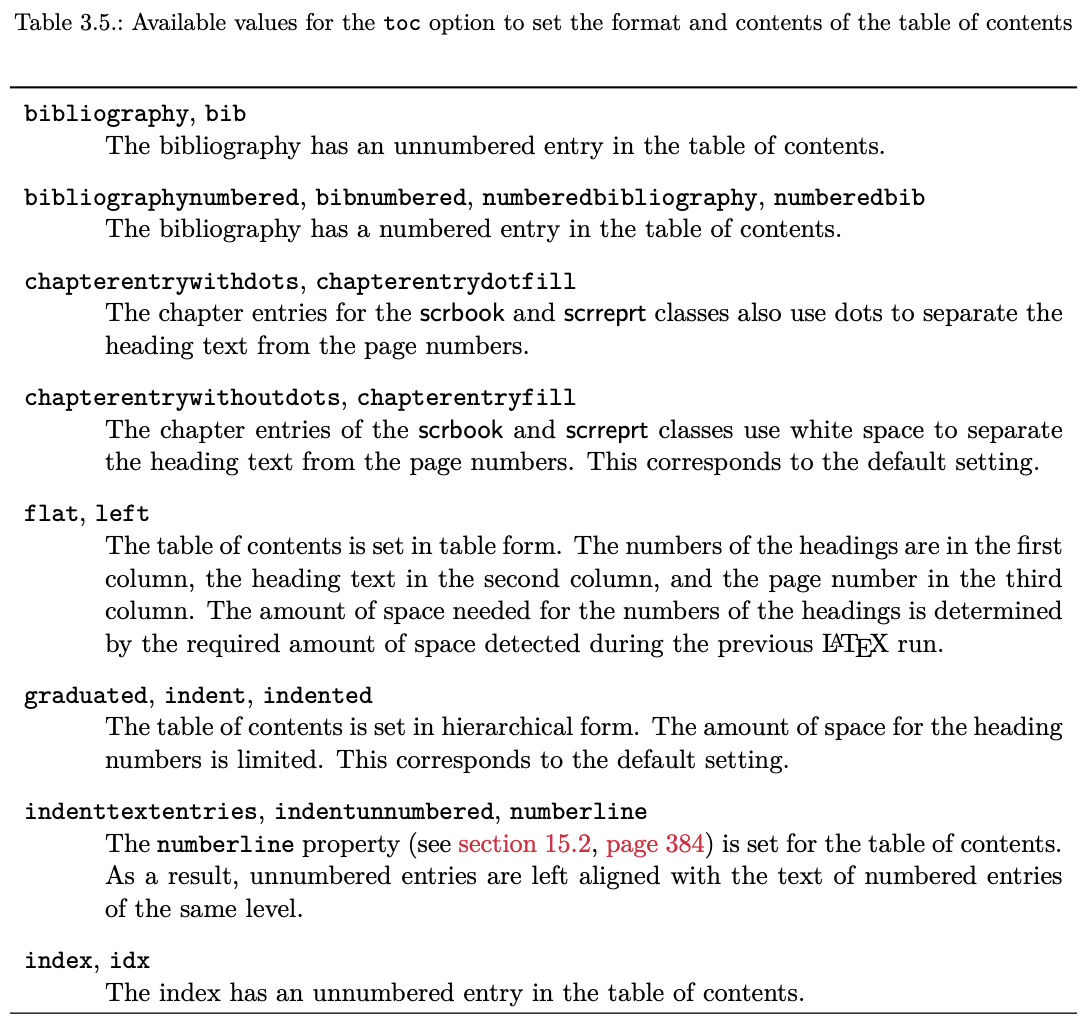
\includegraphics[width=1\linewidth]{tab3_5.png}
    \caption{Tabela 3.5 do Manual}
    \label{fig:tab3_5}
\end{figure}

\begin{figure}
    \centering
    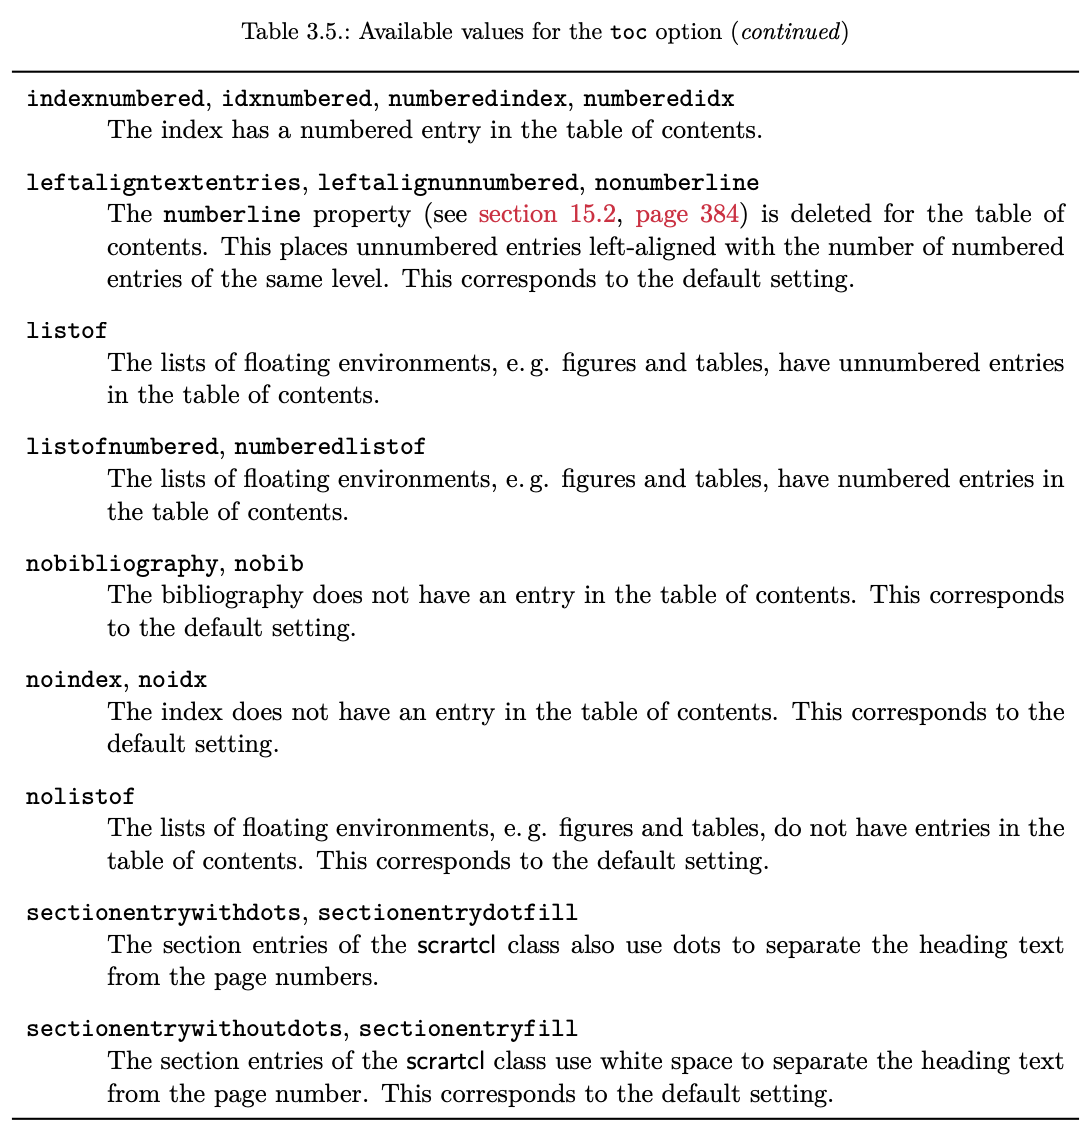
\includegraphics[width=1\linewidth]{tab3_5b.png}
    \caption{Tabela 3.5 do Manual}
    \label{fig:tab3_5b}
\end{figure}

Normalmente, as divisões de seccionamento incluídas no índice são todas aquelas de \verb|\part| para \verb|\subsection| para as classes scrbook e scrreprt, ou de \verb|\part| para \char`\\\texttt{sub\-sub\-sec\-tion} para a classe scrartcl.

Se deve ou não incluir um nível de seccionamento no índice é controlado pelo contador tocdepth. Ele tem o valor -1 para \verb|\part|, 0 para \verb|\chapter|, e assim por diante. Ao incrementar ou decrementar o contador, você pode escolher o menor nível  de seccionamento para incluir no índice. Aliás, as classes padrão funcionam da mesma forma com as classes padrão, com o \KOMAScript\ você não precisa se lembrar dessas formas. Ao contrário dos valores. O \KOMAScript\ define um comando \verb|\level tocdepth| para cada nível de seccionamento com o valor apropriado que você pode usar para definir \verb|tocdepth|.

Observe que em scrartcl, os valores de \verb|tocdepth| e \verb|secnumdepth| (veja a seção 3.16, página 113) para \verb|\part| não são os mesmos. Esse comportamento foi copiado da classe de artigo padrão para compatibilidade. Assim, por exemplo, você não deve usar \char`\\\texttt{part\-num\-depth} para definir o valor de \verb|tocdepth|.

\textbf{Exemplo}: Suponha que você esteja preparando um artigo que usa o sectioning level \char`\\\texttt{sub\-sub\-section}. No entanto, você não quer que esse nível de \textit{sectioning} apareça no índice. O preâmbulo do seu documento pode conter o seguinte:

\begin{verbatim}
    \documentclass{scrartcl}
    \setcounter{tocdepth}{\subsectiontocdepth}
\end{verbatim}

Assim, você define o contador \verb|tocdepth| para o valor do comando \char`\\\texttt{sub\-sec\-tion\-toc\-depth }. Esse valor normalmente é 2, mas dessa forma, você não precisa se lembrar dele.

Se, em vez disso, você simplesmente quiser incluir um nível a menos no índice do que normalmente faria, você pode simplesmente subtrair um do valor padrão de \verb|tocdepth|:
\begin{verbatim}
    \documentclass{scrartcl}
    \addtocounter{tocdepth}{-1}
\end{verbatim}

O valor que você precisa adicionar ou subtrair de tocdepth é listado no índice de conteúdo após pelo menos duas execuções do \LaTeX.


\chapter{Marcação de parágrafos}
As classes padrão normalmente definem parágrafos recuados e sem nenhum espaço vertical entre parágrafos. Esta é a melhor solução ao usar um layout de página regular como os produzidos com o pacote \textbf{typearea}. Se nem recuo nem espaço vertical forem usados, apenas o comprimento da última linha daria ao leitor um guia para a quebra de parágrafo. Em casos extremos, é muito difícil dizer se uma linha está cheia ou não. Além disso, os tipógrafos descobrem que um sinal dado no final do parágrafo é facilmente esquecido no início da próxima linha. Um sinal no início do parágrafo é mais facilmente lembrado. O espaçamento entre parágrafos tem a desvantagem de desaparecer em alguns contextos. Por exemplo, após uma fórmula exibida, seria impossível detectar se o parágrafo anterior continua ou se um novo começa. Além disso, no topo de uma nova página, pode ser necessário olhar para a página anterior para determinar se um novo parágrafo foi iniciado ou não. Todos esses problemas desaparecem ao usar recuo. Uma combinação de recuo e espaçamento vertical entre parágrafos é redundante e, portanto, deve ser evitada. O recuo por si só é suficiente. A única desvantagem do recuo é que ele encurta o comprimento da linha. O uso do espaçamento entre parágrafos é, portanto, justificado ao usar linhas curtas, como em um jornal.

\minisec{parskip=method}
De vez em quando, você pode precisar de um layout de documento com espaçamento vertical entre parágrafos em vez de recuo. As classes \KOMAScript\ fornecem várias maneiras de fazer isso com a opção parskip. O método consiste em dois elementos. O primeiro elemento é \texttt{full} ou \texttt{half}, onde \texttt{full} representa um espaçamento de parágrafo de uma linha e \texttt{half} representa um espaçamento de parágrafo de meia linha. O segundo elemento consiste em um dos caracteres ``$\ast$'', ``$+$'' ou ``$-$'' e pode ser omitido. Sem o segundo elemento, a linha final de um parágrafo terminará com um espaço em branco de pelo menos 1em. Com o caractere mais como o segundo elemento, o espaço em branco terá pelo menos um terço --- e com o asterisco um quarto --- da largura de uma linha normal. Com a variante menos, nenhuma provisão é feita para espaço em branco na última linha de um parágrafo.

Você pode alterar a configuração a qualquer momento. Se você alterá-la dentro do documento, o comando \char`\\\texttt{se\-lect\-font} será chamado implicitamente. Alterações no espaçamento de parágrafos dentro de um parágrafo não serão visíveis até o final do parágrafo.

Além das oito combinações resultantes para o método , você pode usar os valores para interruptores simples mostrado na tabela 2.5, página 41. Ativar a opção corresponde a usar \texttt{full} sem segundo elemento e, portanto, resulta em espaçamento entre parágrafos de uma linha com pelo menos 1em espaço em branco no final da última linha de cada parágrafo. Desativar a opção reativa o recuo padrão de 1em na primeira linha do parágrafo em vez do espaçamento de parágrafo. Um resumo de todos os valores possíveis para o método é mostrado na tabela 3.7.

\begin{figure}[h]
    \centering
    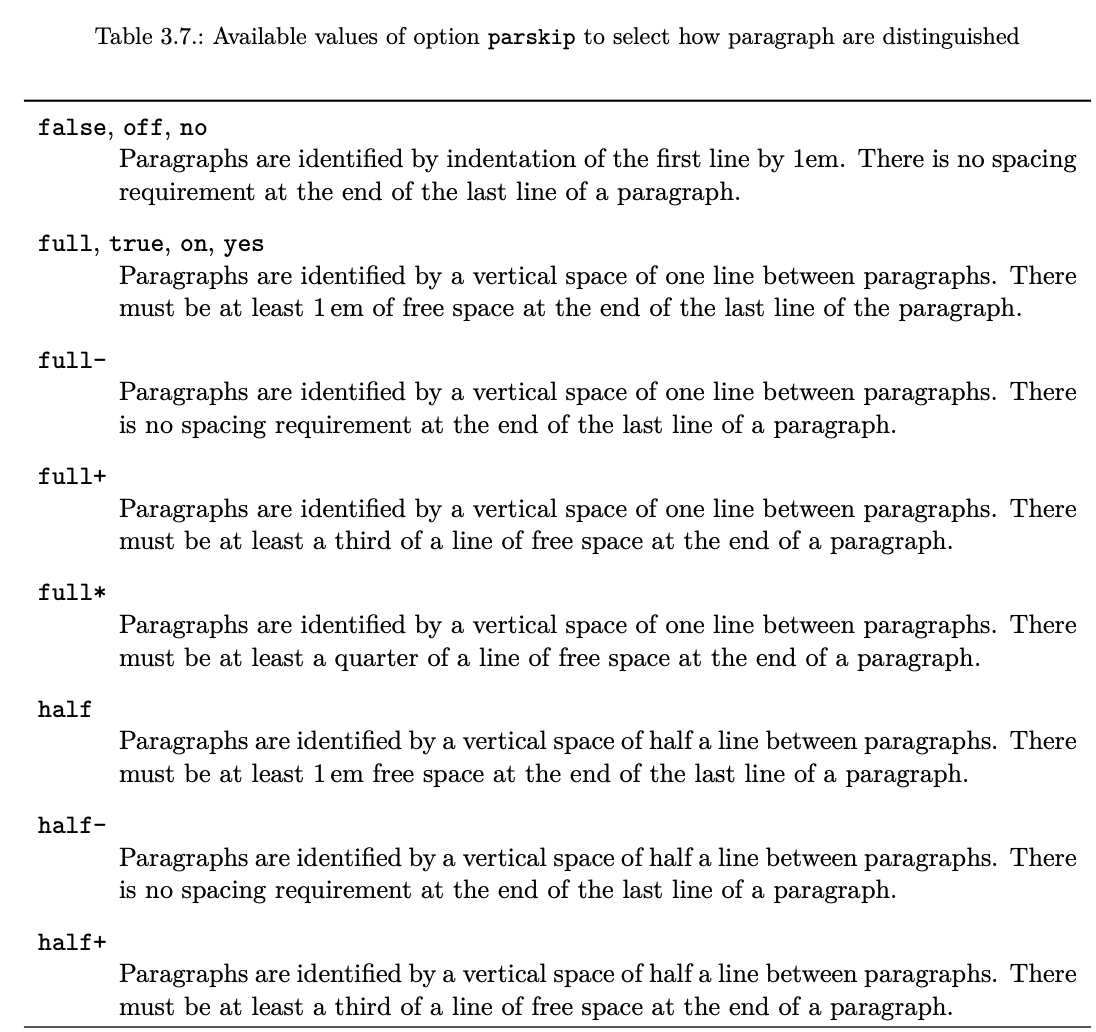
\includegraphics[width=0.9\linewidth]{tab3_7.png}
    \caption{Tabela 3.7 --- Manual}
    \label{fig:tab3_7}
\end{figure}

\begin{figure}[t!]
    \centering
    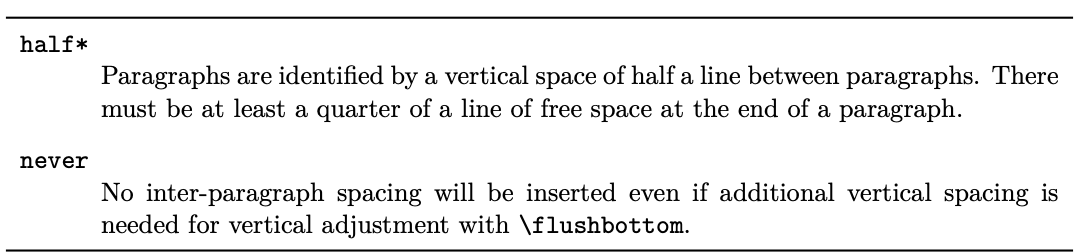
\includegraphics[width=0.8\linewidth]{tab3_7b.png}
    \caption{Tabela 3.7 --- Manual}
    \label{fig:tab3_7b}
\end{figure}

Todos os oito valores de opção \texttt{full} e \texttt{half} também alteram o espaçamento antes, depois e dentro dos ambientes de lista. Isso impede que esses ambientes ou os parágrafos dentro deles tenham uma separação maior do que aquela entre os parágrafos do texto normal. Além disso, essas opções garantem que o índice e as listas de figuras e tabelas sejam definidos sem nenhum espaçamento adicional.

O comportamento padrão do \KOMAScript\ é \texttt{parskip=false}. Nesse caso, não há espaçamento entre parágrafos, apenas um recuo da primeira linha por 1em.

\chapter{Detectando páginas pares e ímpares}
Em documentos de dois lados, distinguimos páginas esquerda e direita. As páginas esquerdas sempre têm um número de página par, e as páginas direitas sempre têm um número de página ímpar. Identificar páginas direitas e esquerdas é equivalente a identificar páginas pares ou ímpares, e por isso normalmente nos referimos a elas como páginas pares e ímpares neste guia.

Em documentos de um lado, a distinção entre páginas esquerda e direita não existe. No entanto, ainda há páginas com números de página pares e ímpares.
\begin{verbatim}
    \Ifthispageodd{true part}{false part}
\end{verbatim}

Se você quiser determinar se o texto aparece em uma página par ou ímpar, o \KOMAScript\ fornece o comando \char`\\\texttt{If\-this\-page\-odd}. O argumento da parte \texttt{true} é executado somente se você estiver atualmente em uma página ímpar. Caso contrário, o argumento da parte \texttt{false} é executado.

\textbf{Exemplo}: Suponha que você simplesmente queira mostrar se um texto será colocado em uma página par ou ímpar. Você pode conseguir isso usando:

Esta página tem um número de página \char`\\\texttt{If\-this\-page\-odd\{odd\}\{even\}}.

Como o comando \verb|\Ifthispageodd| usa um mecanismo muito semelhante a um rótulo e uma referência a ele, pelo menos duas execuções do \LaTeX\ são necessárias após cada alteração no texto. Só então a decisão estará correta. Na primeira execução, uma heurística é usada para fazer a escolha inicial.

Na seção 21.1, página 475, usuários avançados podem encontrar mais informações sobre os problemas de detectar páginas esquerda e direita, ou números de páginas pares e ímpares.

\chapter{Cabeçalhos e Rodapés}
\minisec{Usando Estilos de Página Predefinidos}

Uma das características gerais de um documento é o estilo de página. No \LaTeX, isso consiste principalmente no conteúdo dos cabeçalhos e rodapés.
\begin{verbatim}
        headsepline=simple switch
        footsepline=simple switch
\end{verbatim}

Você pode usar essas opções para especificar se uma regra horizontal aparece abaixo do cabeçalho ou acima do rodapé. Você pode usar qualquer um dos valores para interruptores simples mostrados na tabela 2.5, página 41. Definir a opção \texttt{headsepline} como \texttt{true} ou invocá-la sem valor resulta em uma linha abaixo do cabeçalho. Da mesma forma, ativar a opção \texttt{footsepline} resulta em uma regra acima do rodapé. Desativar qualquer uma das opções desliga a respectiva regra.

A opção \texttt{headsepline} naturalmente não tem efeito com os estilos de página vazio e simples, que são descritos abaixo, porque esses estilos dispensam explicitamente um cabeçalho. Tipograficamente, tal linha tem o efeito de fazer o cabeçalho parecer mais próximo do texto. Isso não significa que o cabeçalho precisa ser movido para mais longe do corpo do texto. Em vez disso, o cabeçalho deve ser considerado como pertencente ao corpo do texto para fins de cálculo da área do tipo. O \KOMAScript\ leva isso em consideração ao passar a \texttt{head\-sep\-li\-ne\-op\-tion} para o pacote \textbf{typearea}, que então executa automaticamente a opção de pacote \texttt{headinclude} com o mesmo valor. O mesmo se aplica à linha de separação do rodapé. Ao contrário do \texttt{headsepline}, a opção \texttt{footsepline} também afeta o estilo de página simples porque \textbf{plain} imprime um número de página no rodapé.

O pacote scrlayer-scrpage (veja capítulo 5) oferece mais possibilidades para ajustar linhas em cabeçalhos e rodapés.
\begin{verbatim}
        \pagestyle{page style}
        \thispagestyle{local page style}
\end{verbatim}

\minisec{Geralmente, há quatro estilos de página diferentes:}
\paragraph{empty} é o estilo de página com cabeçalhos e rodapés completamente vazios. No \KOMAScript\ isso é idêntico às classes padrão.

\paragraph{headings} (títulos) é o estilo de página com títulos correntes no cabeçalho. Neste estilo, os títulos são inseridos automaticamente no cabeçalho. Com as classes scrbook e scrreprt, os títulos de capítulos e seções são repetidos no cabeçalho para impressão frente e verso — no lado externo com \KOMAScript no lado interno com as classes padrão. \KOMAScript\ coloca o número da página no lado externo do rodapé; as classes padrão o colocam no lado interno do cabeçalho. Na impressão de um lado, \KOMAScript\ usa apenas os títulos dos capítulos, que são centralizados no cabeçalho, e coloca os números das páginas centralizados no rodapé. scrartcl se comporta de forma semelhante, mas começa um nível mais abaixo na hierarquia de seções, com seções e subseções, porque o nível do capítulo não existe neste caso.

Enquanto as classes padrão convertem automaticamente os títulos correntes em letras maiúsculas, \KOMAScript\ usa a capitalização encontrada nos títulos. Há várias razões tipográficas para isso. Letras maiúsculas são realmente muito grandes como decoração de texto. Se você usá-las de qualquer maneira, elas devem ser definidas um ponto menor e com espaçamento um pouco mais apertado. As classes padrão não levam esses pontos em consideração.

Além disso, as classes \KOMAScript\ suportam regras abaixo do cabeçalho e acima do rodapé com as opções \texttt{headsepline} e \texttt{footsepline} (veja a página 80).

\paragraph{myheadings} corresponde principalmente ao estilo de página de títulos, mas os títulos correntes não são gerados automaticamente --- eles precisam ser definidos pelo usuário. Você pode usar os comandos \verb|\markboth| e \verb|\markright| para esse propósito (veja a página 83).

\paragraph{Plain} é o estilo de página sem cabeçalho e apenas um número de página no rodapé. As classes padrão sempre centralizam esse número de página no rodapé. \KOMAScript\ coloca o número de página no lado externo do rodapé no modo frente e verso. \KOMAScript\ se comporta como as classes padrão na impressão de um lado.

Você pode definir o estilo da página a qualquer momento com a ajuda do comando \verb|\pagestyle|, e essa configuração entra em vigor na próxima página que for gerada. Se você usar \verb|\pagestyle| logo antes de um comando que resulte em uma quebra de página implícita e se o novo estilo de página deve ser usado na nova página resultante, um \verb|\cleardoublepage| logo antes de \verb|\pagestyle| será útil. Mas normalmente você define o estilo da página apenas uma vez, no início do documento ou no preâmbulo.

Para alterar o estilo da página atual apenas, use o comando \verb|\thispagestyle|. Isso ocorre automaticamente em alguns pontos do documento. Por exemplo, o comando
\begin{verbatim}
        \thispagestyle{\chapterpagestyle}   
\end{verbatim}

é emitido implicitamente na primeira página de um capítulo.
Observe que quando você usa o pacote scrlayer-scrpage, alternar entre cabeçalhos automáticos e manuais não é mais realizado alterando os estilos de página, mas com instruções especiais. Você não deve usar os estilos de página \textbf{headings} e \textbf{myheadings} com este pacote.

Para alterar o estilo de fonte usado para o cabeçalho, rodapé ou número de página, use os comandos \verb|\setkomafont| e \verb|\addtokomafont| (veja a seção 3.6, página 58). O mesmo elemento, pageheadfoot, é usado para o cabeçalho e o rodapé. O elemento para o número de página dentro do cabeçalho ou rodapé é chamado pagenumber. O elemento pagefoot, que também é fornecido pelas classes \KOMAScript é usado somente se você definir um estilo de página com o pacote scrlayer-scrpage no qual o rodapé contém texto (veja capítulo 5, página 264).

Você pode encontrar as configurações padrão na tabela 3.8.

\begin{figure}[h]
    \centering
    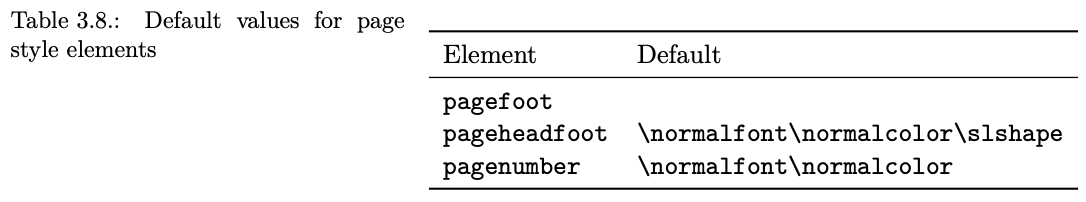
\includegraphics[width=0.8\linewidth]{tab3_8.png}
    \caption{Tabela 3.8 do Manual}
    \label{fig:tab3_8}
\end{figure}

\begin{verbatim}
        \markboth{left mark}{right mark}
        \markright{right mark}
\end{verbatim}

O estilo de página \textbf{myheadings} não define o cabeçalho de execução. Em vez disso, você o define com a ajuda dos comandos \verb|\markboth| e \verb|\markright|. Dessa forma, a marca da esquerda normalmente será usada no cabeçalho de páginas pares e a marca da direita no cabeçalho de páginas ímpares. Com a impressão de um lado, apenas a marca da direita existe. Com o pacote scrlayer-scrpage, o comando \verb|\markleft| também está disponível.

Você pode usar esses comandos com outros estilos de página também. No entanto, quando combinados com cabeçalhos de execução automáticos, por exemplo, com o estilo de página de títulos, o efeito dos comandos dura apenas até a próxima vez que as respectivas marcas forem definidas automaticamente.
\begin{verbatim}
        \titlepagestyle
        \partpagestyle
        \chapterpagestyle
        \indexpagestyle
\end{verbatim}

\begin{figure}[ht]
    \centering
    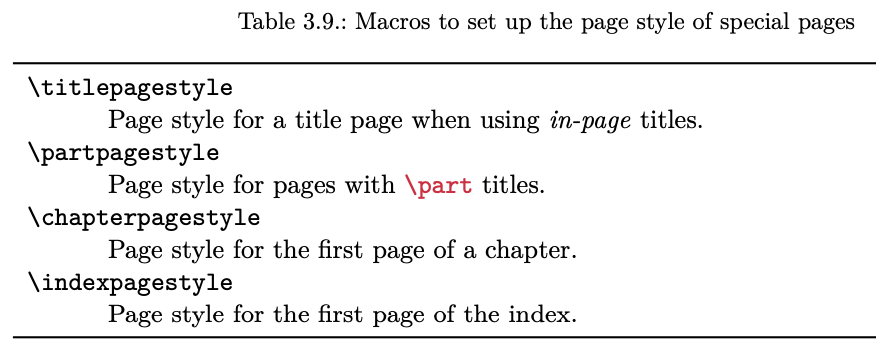
\includegraphics[width=0.75\linewidth]{tab3_9.png}
    \caption{Tabela 3.9 do Manual}
    \label{fig:tab3_9}
\end{figure}

Em algumas páginas, um estilo de página diferente é escolhido automaticamente com a ajuda do comando \verb|\thispagestyle|. Qual estilo de página realmente é, é definido por essas quatro macros, das quais \verb|\partpagestyle| e \verb|\chapterpagestyle| são encontradas apenas com as classes scrbook e scrreprt, e não em scrartcl. O valor padrão para todos os quatro casos é \textbf{plain}. Você pode encontrar o significado dessas macros  na tabela 3.9. Você pode redefinir os estilos de página com a macro \verb|\renewcommand|.

\textbf{Exemplo}: Suponha que você não queira que as páginas com um título \verb|\part| sejam numeradas. Você pode usar o seguinte comando no preâmbulo do seu documento:
\begin{verbatim}
    \renewcommand*{\partpagestyle}{empty}
\end{verbatim}

Conforme mencionado anteriormente na página 80, o estilo de página vazio é exatamente o que é necessário neste exemplo. Claro, você também pode usar um estilo de página definido pelo usuário.

\minisec{\char`\\\texttt{pagenumbering\{numbering style\}}}

Este comando funciona da mesma forma no \KOMAScript\ como nas classes padrão. Estritamente falando, não é um recurso nem das classes padrão nem das classes \KOMAScript\ mas do kernel \LaTeX. Este comando é usado para alterar o estilo de numeração dos números de página.

As alterações entram em vigor imediatamente, ou seja, a partir da página que contém o comando. Se necessário, você deve primeiro fechar a página atual com \char`\\\texttt{clear\-page} ou melhor \char`\\\texttt{clear\-dou\-ble\-odd\-page}. Você pode encontrar as configurações disponíveis para o estilo de numeração na tabela 3.10.

\begin{figure}[hb]
    \centering
    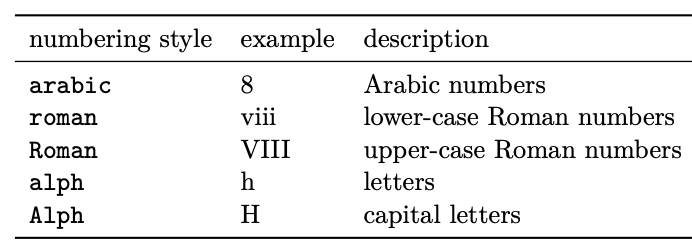
\includegraphics[width=0.7\linewidth]{tab3_10.png}
    \caption{Tabela 3.10 do Manual}
    \label{fig:tab3_10}
\end{figure}

Chamar \verb|\pagenumbering| sempre redefine o número da página. A página atual se torna o número 1 no estilo de numeração selecionado (\textit{numbering style}). Para que documentos frente e verso produzam os resultados corretos em uma página par, para que a página da esquerda não esteja faltando, você deve sempre adicionar \char`\\\texttt{clear\-dou\-ble\-odd\-pa\-ge} antes de \char`\\\texttt{pa\-ge\-num\-be\-ring}. A próxima seção fornece mais informações sobre páginas em branco potencialmente inseridas.

Deixe-me dizer uma palavra sobre um erro comum encontrado em vários modelos que circulam na Internet. Se você encontrar linhas como a seguinte — sem o comentário inicial, naturalmente — este é um sinal inequívoco de que o criador não leu ou entendeu a observação acima:
\begin{verbatim}
        % Atenção! Este exemplo contém erros!
        % Observe a explicação no texto!
        \tableofcontents
        \pagenumbering{arabic}
        \setcounter{page}{1}
\end{verbatim}

Como \verb|\tableofcontents| gera o índice, mas não emite automaticamente uma quebra de página no final, a numeração de página já foi alterada na última página do índice. Como não tem um comando \char`\\\texttt{clear\-dou\-ble\-odd\-pa\-ge} antes de \char`\\\texttt{pa\-ge\-num\-be\-ring}, ele recebe uma paginação do número arábico 1. Além disso, a linha final que define a numeração de página para 1 é supérflua, pois isso já é feito por \char`\\\texttt{pa\-ge\-num\-be\-ring}.

Às vezes --- sem o comentário inicial, naturalmente --- você encontra:
\begin{verbatim}
        % Atenção! Este exemplo contém erros!
        % Observe a explicação no texto!
        \tableofcontents
        \pagebreak
        \pagenumbering{arabic}
        \setcounter{page}{1}
\end{verbatim}

Aqui, o criador tentou resolver o problema com a página final do índice com a ajuda de \char`\\\texttt{pa\-ge\-break}

Infelizmente, esta solução não é muito melhor. Aqui, há uma quebra de página após a última página do índice. Isso pode fazer com que as entradas na última página de um documento frente e verso tenham espaçamento vertical excessivo (consulte \char`\\\texttt{flush\-bot\-tom}, página 57). \char`\\\texttt{pa\-ge\-break} é claramente o comando errado aqui.

Além disso, \verb|\newpage| ou \char`\\\texttt{clear\-pa\-ge} não seriam suficientes para um documento frente e verso. Por exemplo, se a última página do índice tivesse o numeral romano \textit{vii}, a página direita numerada arábica 1 seguiria imediatamente a página direita numerada romana. Uma página esquerda entre as duas estaria faltando, o que poderia causar sérios problemas com a impressão posterior.

Meu conselho: Evite usar modelos que contenham erros com relação a coisas tão simples. Aliás, a maneira correta seria:
\begin{verbatim}
    \tableofcontents
    \cleardoubleoddpage
    \pagenumbering{arabic}
\end{verbatim}

Isso também se aplica se \textbf{scrartcl} usa uma classe que normalmente não inicia uma nova página após o índice. Se você alternar a numeração de páginas, uma nova página à direita deve ser iniciada. Se você não quiser tal alteração, você deve manter o estilo de numeração das páginas consistente em todo o documento sem alterá-lo entre elas. É mais fácil alterar o estilo de numeração ao usar \textbf{scrbook}. Lá você tem o suporte de dois comandos, \char`\\\texttt{front\-matter} e \char`\\\texttt{main\-matter}, para a alternância mais comumente usada. Para mais informações, consulte a seção 3.15, página 94.

\chapter[Interleaf Pages]{Interleaf Pages (Páginas Intercaladas)}

Páginas intercaladas são páginas que são inseridas entre partes de um documento. Tradicionalmente, essas páginas são completamente em branco. O \LaTeX, no entanto, as define por padrão com o estilo de página atual. O \KOMAScript\ fornece várias extensões para essa funcionalidade.

Páginas intercaladas são encontradas principalmente em livros. Como os capítulos de livros geralmente começam na página direita (frente) de uma página dupla, uma página esquerda (verso) vazia deve ser inserida se o capítulo anterior terminar em uma página frente. Por esse motivo, as páginas intercaladas realmente só existem para impressão frente e verso.
\begin{center}
    
\includegraphics[width=0.5\linewidth]{imagem15.png}
\end{center}
Com esta opção, você pode definir o estilo de página das páginas intercaladas criadas pelos comandos \char`\\\texttt{clear\-dou\-ble\-pa\-ge} \char`\\\texttt{clear\-dou\-ble\-odd\-pa\-ge}  ou \char`\\\texttt{clear\-dou\-ble\-e\-ven\-pa\-ge} para avançar para a página desejada. Você pode usar qualquer estilo de página definido anteriormente (consulte a seção 3.12 da página 80 e capítulo 5 da página 255). Além disso, \texttt{clear\-dou\-ble\-pa\-ge=cur\-rent} também é possível. Este caso corresponde ao padrão anterior ao \KOMAScript~2.98c e cria uma página intercalada sem alterar o estilo da página. A partir do \KOMAScript~3.00, o padrão segue a recomendação da maioria dos tipógrafos e cria páginas intercaladas com o estilo de página vazio, a menos que você altere a compatibilidade para versões anteriores do \KOMAScript\ (consulte a opção versão, seção 3.2, página 55).

\textbf{Exemplo}: Suponha que você queira páginas intercaladas que estejam vazias, exceto pela paginação, para que elas sejam criadas com \texttt{plain}. Você pode conseguir isso, por exemplo, com:

\begin{verbatim}
        \KOMAoptions{cleardoublepage=plain}
\end{verbatim}

Você pode encontrar mais informações sobre o estilo de página simples (\textbf{plain page style}) na seção 3.12, página 81.

O kernel do \LaTeX\ fornece o comando \verb|\clear\-page|, que garante que todos os \textbf{floats} pendentes sejam exibidos e então inicie uma nova página. Há também o comando \char`\\\texttt{clear\-dou\-ble\-pa\-ge}, que funciona como \verb|\clear\-page|, mas que inicia uma nova página à direita na impressão frente e verso (veja a opção de layout frente e verso na seção 2.4, página 40). Uma página vazia à esquerda no estilo de página atual é exibida, se necessário.

\begin{figure}[hb]
    \centering
    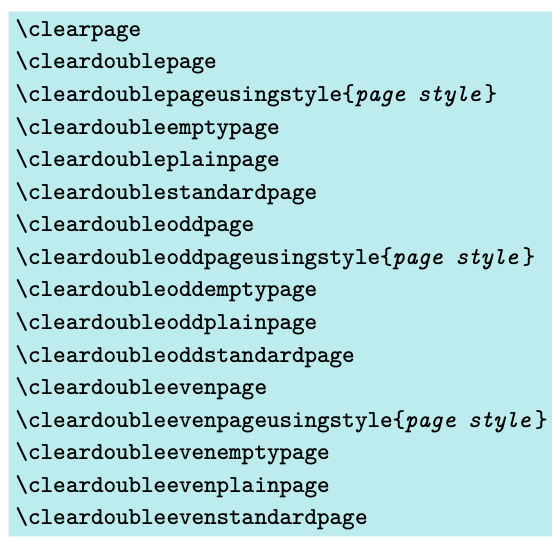
\includegraphics[width=0.75\linewidth]{imagem16.png}
    %\caption{Enter Caption}
    \label{fig:img16}
\end{figure}


    

\chapter{Estrutura do livro}
Às vezes, os livros são vagamente divididos em matéria frontal, matéria principal e matéria final. O \KOMAScript\ também fornece essa capacidade para \textbf{scrbook}.
\begin{verbatim}
        \frontmatter
        \mainmatter
        \backmatter
\end{verbatim}

A matéria frontal inclui todo o material que aparece antes do texto principal começar, incluindo páginas de título, prefácio e índice. Ele é iniciado com \verb|\frontmatter|. Na matéria frontal, algarismos romanos são usados para os números de página, e os títulos dos capítulos no cabeçalho não são numerados. No entanto, os títulos das seções são numerados consecutivamente, começando do capítulo 0. Isso normalmente não importa, pois a matéria frontal é usada apenas para as páginas de título, índice de conteúdo, listas de figuras e tabelas e um prefácio ou prefácio. O prefácio pode, portanto, ser criado como um capítulo normal. Um prefácio deve ser o mais curto possível e nunca dividido em seções. O prefácio, portanto, não requer um nível mais profundo de estrutura do que o capítulo.

Se você vê as coisas de forma diferente e deseja usar seções numeradas nos capítulos da matéria frontal, a partir da versão $2.97e$, a numeração da seção não contém mais o número do capítulo. Esta alteração só entra em vigor quando a opção de compatibilidade é definida para pelo menos a versão $2.97e$ (veja a opção versão, seção 3.2, página 55). É explicitamente notado que isso cria confusão com números de capítulos! O uso de \verb|\addsec| e \verb|\section*| (veja a seção 3.16, página 105 e página 106) são, portanto, na opinião do autor, muito preferíveis.

A partir da versão $2.97e$ a numeração de ambientes flutuantes, como tabelas e figuras, e números de equações no \textbf{front matter} também não contém nenhuma parte de número de capítulo. Para entrar em vigor, isso também requer a configuração de compatibilidade correspondente (veja a opção versão, seção 3.2, página 55).

A parte do livro com o texto principal é introduzida com \char`\\\texttt{main\-matter}. Se não houver \textbf{front matter}, você pode omitir este comando. A numeração de páginas padrão no \textbf{main matter} usa algarismos arábicos e (re)inicia a contagem de páginas em 1 no início do \textbf{main matter}.

O \textbf{back matter} é introduzido com \verb|\backmatter|. As opiniões diferem quanto ao que pertence ao \textbf{back matter}. Então, em alguns casos, você encontrará apenas a bibliografia, em alguns casos, apenas o índice e, em outros casos, ambos, bem como os apêndices. Os capítulos no\textbf{ back matter} são semelhantes aos capítulos no\textbf{ front matter}, mas a numeração de páginas não é redefinida. Se você precisar de numeração de páginas separada, pode usar o comando \verb|\pagenumbering| na seção 3.12, página 85.

\chapter{Estrutura do documento}
A estrutura se refere à divisão de um documento em partes, capítulos, seções e níveis adicionais de estrutura.
\begin{figure}[h]
    \centering
    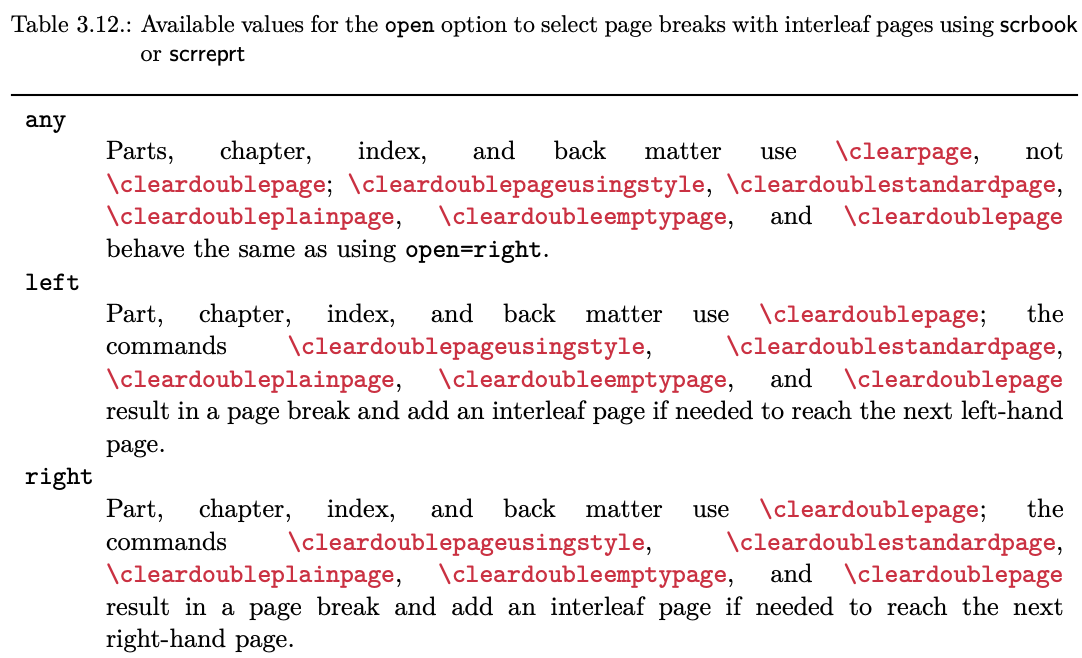
\includegraphics[width=0.80\linewidth]{imagem17.png}
    %\caption{Enter Caption}
    \label{fig:3_12}
\end{figure}

\minisec{open=method}
As classes \KOMAScript\ \texttt{scrbook} e \texttt{scrreprt} oferecem a você a opção de onde começar um novo capítulo com impressão frente e verso. Por padrão, \texttt{scrreprt} inicia um novo capítulo na próxima página. Isso é equivalente ao método any. No entanto, \texttt{scrbook} inicia novos capítulos na próxima página à direita. Isso é equivalente ao método right e geralmente é usado em livros. Mas às vezes os capítulos devem começar na página esquerda de uma página dupla. Você pode fazer isso com o método left. Você pode encontrar um resumo dos valores disponíveis na tabela 3.12. A tabela também descreve os efeitos de \char`\\\texttt{clear\-dou\-ble\-pa\-ge}, \char`\\\texttt{clear\-dou\-ble\-pa\-ge\-u\-sing\-sty\-le}, \char`\\\texttt{clear\-dou\-ble\-stan\-dard\-pa\-ge}, \char`\\\texttt{clear\-dou\-ble\-plain\-pa\-ge} e \char`\\\texttt{clear\-dou\-ble\-empty\-pa\-ge} (consulte a seção 3.13, página 87).

Como o \LaTeX\ não diferencia entre páginas esquerdas e direitas na impressão de um lado, a opção não tem efeito nesse caso.

Na classe \texttt{scrartcl}, a seção é o primeiro elemento estrutural abaixo da peça. Por esse motivo, \texttt{scrartcl} não suporta essa opção.

\begin{figure}
    \centering
    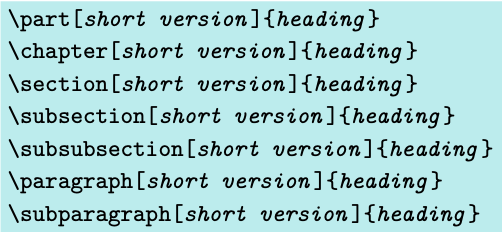
\includegraphics[width=0.65\linewidth]{imagem18.png}
    \label{fig:img18}
\end{figure}

Os comandos de seccionamento padrão no \KOMAScript\ funcionam da mesma forma que aqueles nas classes padrão. Assim, você pode especificar um texto alternativo para o índice e títulos como um argumento opcional para os comandos de seccionamento.

No entanto, com a opção \texttt{headings=optiontohead}, o \KOMAScript\ usa apenas a versão curta do argumento opcional no título, não no índice. Claro, esse texto só aparecerá se você usar um estilo de página que coloque o nível de seccionamento correspondente no título. Veja a seção 3.12 e o capítulo 5. Com a opção \texttt{headings=optiontotoc}, o \KOMAScript\ usa a versão curta (\textit{short version}) do argumento opcional exclusivamente para o índice e não para o título. No entanto, a entrada será mostrada apenas se o \texttt{tocdepth counter} for grande o suficiente (veja a seção 3.9, página 76). Com a opção \texttt{headings=optiontoheadandtoc}, o \KOMAScript\ usa a versão curta do argumento opcional tanto no índice quanto no título. Todas essas três opções ativam a interpretação estendida da versão curta do argumento opcional, que não está ativa por padrão.

A interpretação estendida do argumento opcional verifica se há um sinal de igual na versão curta. Se houver, o argumento opcional será interpretado como uma lista de opções. Quatro opções
\begin{itemize}
    \item \texttt{head=running head},
    \item \texttt{tocentry=table of contents entry},
    \item \texttt{reference=reference title} e 
    \item \texttt{nonumber=simple switch}
\end{itemize}

são suportadas com este formato. Para usar vírgulas ou sinais de igual dentro dos valores dessas opções, você deve colocá-los entre chaves.

Observe que este mecanismo só funciona enquanto o \KOMAScript\ controlar os comandos de seccionamento. Se você usar um pacote que redefine os comandos de seccionamento do \KOMAScript\ ou do kernel interno do \LaTeX, o \KOMAScript\ não poderá mais fornecer este mecanismo estendido. Isso também se aplica a uma extensão do \KOMAScript\ que está sempre ativa: comandos de seccionamento sem texto de título não criam entradas no índice. Se você realmente quiser uma entrada com texto de título vazio, você pode usar uma entrada invisível como \mbox{}.

\textbf{Exemplo}: Suponha que você tenha um documento com títulos de capítulo muito longos. Esses títulos devem aparecer no índice, mas você quer limitar o título corrente a títulos curtos de uma única linha. Você pode fazer isso com o argumento opcional de \char`\\\texttt{chap\-ter}.

\begin{figure}[h]
    \centering
    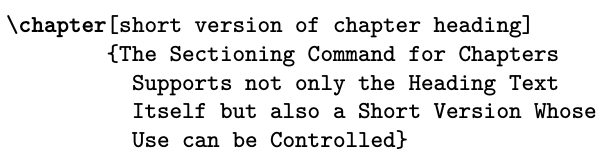
\includegraphics[width=0.60\linewidth]{imagem14.png}
    \label{fig:img14}
\end{figure}

Um pouco mais tarde, você percebe que as quebras de linha para esse longo título são muito inapropriadas. Portanto, você quer escolher as quebras você mesmo. No entanto, você ainda quer quebra de linha automática no índice. Com
\begin{figure}[h]
    \centering
    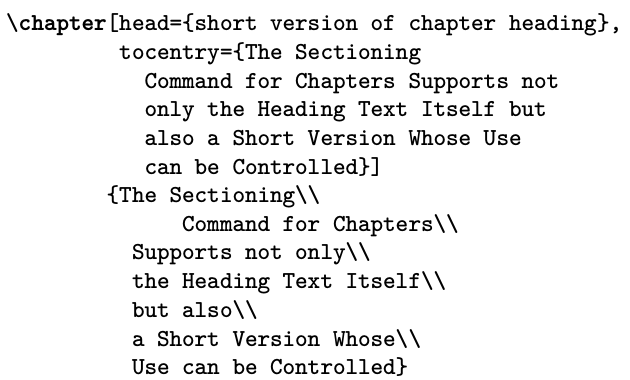
\includegraphics[width=0.60\linewidth]{imagem19.png}
    %\caption{Enter Caption}
    \label{fig:img19}
\end{figure}

você cria entradas separadas para o índice, título corrente e o próprio título do capítulo. Os argumentos das opções head e tocentry foram colocados entre chaves para que seus conteúdos possam ser arbitrários.

É possível usar diferentes tipos de fonte para diferentes níveis de seccionamento no KOMA-Script. Não especialistas em tipografia devem evitar fazer isso por excelentes razões tipográficas.

Uma regra da tipografia afirma que você deve misturar o mínimo de fontes possível. Usar \textit{sans serif} para títulos já parece violar essa regra. No entanto, você deve perceber que letras grandes, em negrito e \textit{serif} são muito pesadas para títulos. A rigor, você deve usar uma fonte normal em vez de uma fonte em negrito ou seminegrito. No entanto, em níveis mais profundos do seccionamento, uma fonte normal pode então parecer muito clara. Por outro lado, fontes \textit{sans serif} têm uma aparência muito agradável em títulos, e quase exclusivamente em títulos. Há, portanto, uma boa razão pela qual \textit{sans serif} é o padrão no \KOMAScript.


\includegraphics[width=0.40\linewidth]{imagem20.png}

As variantes com estrela de todos os comandos de seccionamento produzem títulos não numerados que não aparecem no índice ou no cabeçalho contínuo. A ausência de um cabeçalho contínuo geralmente tem um efeito colateral indesejado. Se, por exemplo, um conjunto de capítulos usando \verb|\chapter*| abrange várias páginas, então o cabeçalho contínuo do capítulo anterior reaparece repentinamente. O \KOMAScript\ oferece uma solução para esse problema, descrita abaixo. \verb|\chapter*| só existe nas classes book e report, ou seja, book, scrbook, report e scrreport, não nas classes article e scrartcl.

Observe que \verb|\part| e \verb|\chapter| alteram o estilo de página para uma página. Enquanto as classes padrão usam o estilo de página simples, o \KOMAScript\ aplica o estilo definido nas macros \char`\\\texttt{part\-pa\-ge\-sty\-le} e \char`\\\texttt{chap\-ter\-pa\-ge\-sty\-le} (veja a seção 3.12, página 83).

As possibilidades de troca de fontes mudam. Os elementos usam os mesmos nomes, pois não indicam variantes, mas níveis de estruturação.

\section{Minisec}
\begin{verbatim}
   \minisec{heading} 
\end{verbatim}

Às vezes, você quer um título que seja destacado, mas também intimamente vinculado ao texto seguinte. Tal título não deve ser separado por um grande salto vertical.

O comando \verb|\minisec| é projetado para esta situação. Este título não é associado a nenhum nível de seccionamento. Tal minisseção não produz uma entrada no índice, nem recebe nenhuma numeração.

Você pode alterar a fonte do comando \verb|\minisec| usando o elemento \texttt{disposition} e \texttt{minisec} (veja a tabela 3.2, página 59). O padrão do elemento \texttt{minisec} é vazio, então por padrão somente o elemento \texttt{disposition} é usado.

\textbf{Exemplo}: Você desenvolveu um kit para construir uma ratoeira e quer a documentação separada em uma lista de itens necessários e uma descrição de montagem. Você pode escrever o seguinte:

\begin{figure}
    \centering
    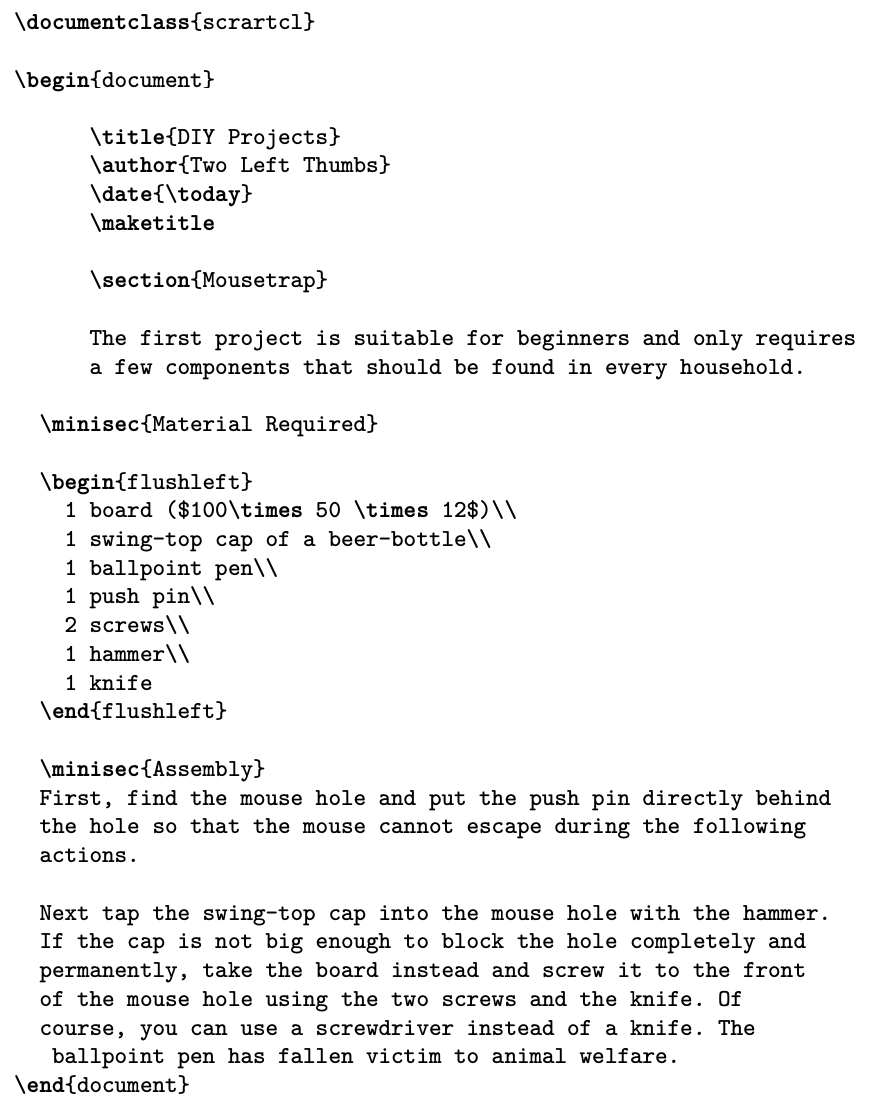
\includegraphics[width=0.8\linewidth]{imagem21.png}
    %\caption{Enter Caption}
    \label{fig:img21}
\end{figure}

\begin{figure}
    \centering
    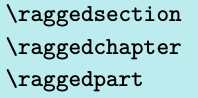
\includegraphics[width=0.4\linewidth]{imagens/imagem22.png}
\end{figure}

\newpage

Nas classes padrão, os títulos são definidos como texto justificado. Isso significa que palavras hifenizadas podem ocorrer e títulos de várias linhas são esticados até a largura do texto. Essa abordagem é bastante incomum em tipografia. O \KOMAScript\ portanto, define os títulos alinhados à esquerda com recuo deslocado usando \char`\\\texttt{ragged\-sec\-tion} com o padrão:
\begin{verbatim}
    \newcommand*{\raggedsection}{\raggedright}
\end{verbatim}

Você pode redefinir este comando com \char`\\\texttt{renewcommand}.

\textbf{Exemplo}: você prefere títulos justificados, então você escreve no preâmbulo do seu documento:
\begin{verbatim}
    \renewcommand*{\raggedsection}{}
\end{verbatim}
ou mais compactamente:
\begin{verbatim}
    \let\raggedsection\relax
\end{verbatim}

Você obterá uma formatação de título muito próxima daquela das classes padrão. Ela ficará ainda mais próxima quando você combinar essa alteração com a alteração no elemento de disposição mencionado acima.

Porque alguns usuários querem um alinhamento diferente para o nível \verb|\chapter| do que para os outros níveis de seção, você pode alterar a justificação \verb|\chapter| separadamente redefinindo \char`\\\texttt{rag\-ged\-chap\-ter}. Por padrão, no entanto, este comando simplesmente usa \char`\\\texttt{rag\-ged\-sec\-tion}, então alterar \char`\\\texttt{rag\-ged\-sec\-tion} afeta indiretamente \char`\\\texttt{rag\-ged\-chap\-ter}.

Por padrão, os títulos de parte (\verb|\part|) são definidos horizontalmente centralizados em vez de irregulares à direita. Esta formatação é realizada pela declaração \verb|\raggedpart|, que tem a definição padrão
\begin{verbatim}
    \let\raggedpart\centering
\end{verbatim}


Você também pode redefinir este comando usando \verb|\renewcommand|.

\textbf{Exemplo}: Você quer que os títulos para \verb|\part| sejam formatados da mesma forma que qualquer outro comando de seção. Para fazer isso, coloque
\begin{verbatim}
    \renewcommand*{\raggedpart}{\raggedsection}
\end{verbatim}

no preâmbulo do seu documento. Neste caso, e diferente do exemplo acima, nós não usamos \verb|\let| porque \verb|\let| definiria \char`\\\texttt{rag\-ged\-part} para o valor subjacente de \char`\\\texttt{rag\-ged\-sec\-tion}. Alterações subsequentes em \char`\\\texttt{rag\-ged\-sec\-tion} não mudariam o comportamento de \char`\\\texttt{rag\-ged\-part}. Ao redefinir com \char`\\\texttt{re\-new\-com\-mand}, \char`\\\texttt{rag\-ged\-part} usará o significado atual de \verb|\raggedsection| no momento em que for usado, em vez de quando foi redefinido.

\begin{figure}
    \centering
    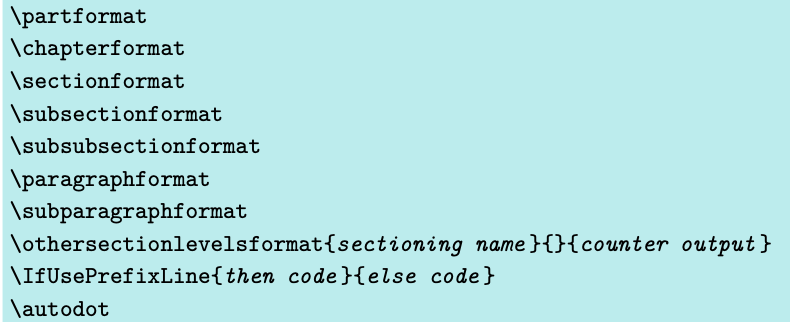
\includegraphics[width=0.8\linewidth]{imagem23.png}
\end{figure}

O \KOMAScript\ adiciona outra camada lógica acima do nome \char`\\\texttt{the\-sec\-tio\-ning} para formatar os números de seccionamento. Os contadores para cada título não são meramente emitidos. Eles são formatados usando os comandos \char`\\\texttt{part\-for\-mat}, \char`\\\texttt{chap\-ter\-for\-mat}, até \char`\\\texttt{sub\-pa\-ra\-graph\-for\-mat}. Claro, o comando \char`\\\texttt{chap\-ter\-for\-mat}, como \verb|\thechapter|, não existe na classe scrartcl, mas apenas nas classes scrbook e scrreprt.

Como já explicado para a opção numbers no início desta seção (veja a página 99), o tratamento de pontos do \KOMAScript\ em números de seção implementa as regras fornecidas em [DUD96], que são padrão na tipografia de língua alemã, no comando \verb|\autodot|. Em todos os níveis exceto para \verb|\part|, um ponto é seguido por um \verb|\enskip| adicional. Isso corresponde a um salto horizontal de 0.5em.

\chapter{Versos}
\begin{verbatim}
        \begin{verse}...\end{verse}    
\end{verbatim}

O ambiente de verso normalmente não é percebido como um ambiente de lista porque você não trabalha com comandos \verb|\item|. Em vez disso, quebras de linha fixas são usadas dentro do ambiente \texttt{flushleft}. Internamente, no entanto, tanto as classes padrão quanto o \KOMAScript\ implementam ele como um ambiente de lista.

Em geral, o ambiente de verso é usado para poesia. As linhas são recuadas tanto à esquerda quanto à direita. Linhas individuais de verso são finalizadas por uma quebra de linha fixa: \verb|\\|. Os versos são definidos como parágrafos, separados por uma linha vazia. Frequentemente, também \verb|\medskip| ou \verb|\bigskip| são usados. Para evitar uma quebra de página no final de uma linha de verso, você pode, como de costume, inserir \verb|\\*| em vez de \verb|\\|.

\textbf{Exemplo}: Como exemplo, o soneto de Emma Lazarus do pedestal de Liberty Enlightening the World:
\begin{verbatim}
\begin{verse}
Not like the brazen giant of Greek fame\\*
With conquering limbs astride from land to land\\*
Here at our sea-washed, sunset gates shall stand\\*
A mighty woman with a torch, whose flame\\*
Is the imprisoned lightning, and her name\\*
Mother of Exiles. From her beacon-hand\\*
Glows world-wide welcome; her mild eyes command\\*
The air-bridged harbor that twin cities frame.\\*
‘‘Keep, ancient lands, your storied pomp!’’ cries she\\*
With silent lips. ‘‘Give me your tired, your poor,\\*
Your huddled masses yearning to breathe free,\\*
The wretched refuse of your teeming shore.\\*
Send these, the homeless, tempest-tossed to me:\\*
I lift my lamp beside the golden door.’’
\end{verse} 
\end{verbatim}

No entanto, se você tiver linhas muito longas de verso onde uma quebra de linha ocorre dentro de uma linha de verso:
\newpage

\begin{verbatim}
\begin{verse}
Both the philosopher and the house-owner
always have something to repair.\\*
\bigskip
Don’t trust a man, my son, who tells you
that he has never lied.
\end{verse}
\end{verbatim}


\chapter{Ambiente Quote/Quotation}
\begin{verbatim}
    \begin{quotation}...\end{quotation}  
\end{verbatim}
Esses dois ambientes também são definidos internamente como ambientes de lista e podem ser encontrados em ambas as classes \textbf{standard} e \KOMAScript. Ambos os ambientes usam texto justificado que é recuado tanto no lado esquerdo quanto no direito. Frequentemente, eles são usados para separar citações mais longas do texto principal. A diferença entre os dois está na maneira como os parágrafos são compostos. Enquanto os parágrafos de citação são distinguidos pelo espaço vertical, nos parágrafos de citação, a primeira linha é recuada. Isso também se aplica à primeira linha de um \texttt{quo\-te\-en\-vi\-ron\-ment}, a menos que seja precedido por \verb|\noindent|.

\chapter{Ambiente Addmargin}

\begin{verbatim}
\begin{addmargin}[left indentation ]{indentation }...\end{addmargin}
\begin{addmargin*}[inner indentation]{indentation }...\end{addmargin*}
\end{verbatim}

Assim como quote e \texttt{quotation}, o ambiente \texttt{addmargin} altera a margem. No entanto, diferentemente dos dois primeiros ambientes, \texttt{addmargin} permite que o usuário altere a largura do recuo. Além desta alteração, este ambiente não altera o recuo da primeira linha nem o espaçamento vertical entre parágrafos.

Se apenas o argumento obrigatório \texttt{indentation} for fornecido, as margens esquerda e direita serão expandidas por este valor. Se o argumento opcional \texttt{left indentation} também for fornecido, então o valor left indentation será usado para a margem esquerda em vez de \texttt{indentation}.

A variante com estrela \texttt{addmargin*} difere da versão normal apenas no modo de dois lados. Além disso, a diferença só ocorre se o argumento opcional \texttt{inner indentation} for usado. Neste caso, o valor de \texttt{inner indentation} é adicionado ao recuo interno normal. Para páginas à direita, esta é a margem esquerda; para páginas à esquerda, a margem direita. Então o valor de \texttt{indentation} determina a largura da margem oposta.

Ambas as versões deste ambiente permitem valores negativos para todos os parâmetros. Isso pode ser feito para que o ambiente se projete para a margem.

\chapter{``Floats'' para Tabelas e Figuras}
Com os ambientes flutuantes, o \LaTeX\ oferece um mecanismo poderoso e conveniente para organizar figuras e tabelas automaticamente. Frequentemente, iniciantes não entendem corretamente esses ambientes flutuantes. Eles geralmente pedem para especificar a posição exata de uma tabela ou figura dentro do texto. No entanto, isso geralmente é desnecessário, pois o texto conterá referências a esses ambientes flutuantes. Também não é sensato porque tal objeto só pode ser definido na página se houver espaço suficiente para ele. Se esse não for o caso, o objeto teria que ser deslocado para a próxima página, possivelmente deixando um enorme espaço vazio na página anterior.

Frequentemente, um documento usará o mesmo argumento opcional para posicionar cada objeto flutuante. Isso também não faz sentido. Em tais casos, você deve alterar o valor padrão globalmente.

Uma nota final importante antes de começar esta seção: a maioria dos mecanismos descritos aqui, que estendem os recursos das classes padrão, não funcionam mais corretamente quando usados com pacotes que modificam a aparência das legendas de figuras e tabelas. Isso deveria ser evidente, mas é frequentemente esquecido.

\begin{figure}[h]
    \centering
    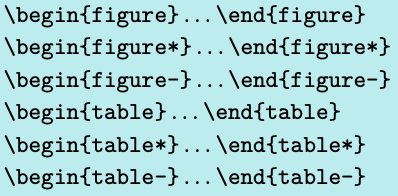
\includegraphics[width=0.5\linewidth]{imagem24.png}
\end{figure}
\chapter{Marginal Notes}
Além da área de texto, que normalmente preenche a área de tipo, os documentos geralmente contêm uma coluna para marginália. Você pode definir notas marginais nesta área. Este guia faz uso frequente delas.

\begin{figure}[h]
    \centering
    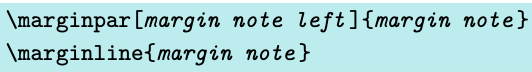
\includegraphics[width=0.6\linewidth]{imagem25.png}
\end{figure}

As notas marginais no \LaTeX\ são geralmente inseridas com o comando \verb|\marginpar|. Elas são colocadas na margem externa. Documentos de um lado usam a borda direita. Embora você possa especificar uma nota marginal diferente para \verb|\marginpar| caso ela acabe na margem esquerda, as notas marginais são sempre totalmente justificadas. No entanto, a experiência mostrou que muitos usuários preferem notas marginais justificadas à esquerda ou à direita. Para esse propósito, o \KOMAScript\ oferece o comando \char`\\\texttt{mar\-gin\-li\-ne}.

\textbf{Exemplo}: Em algumas partes deste guia, o nome da classe scrartcl pode ser encontrado na margem. Você pode produzir isso com:
\begin{verbatim}
    \marginline{\texttt{scrartcl}}   
\end{verbatim}

Em vez de \verb|\marginline|, você poderia ter usado \char`\\\texttt{mar\-gin\-par}. Na verdade, o primeiro comando é implementado internamente como:
\begin{verbatim}
    \marginpar[\raggedleft\texttt{scrartcl}]
    {\raggedright\texttt{scrartcl}}
\end{verbatim}

Assim, \verb|\marginline| é realmente apenas uma notação abreviada para o código acima.

Usuários avançados encontrarão notas sobre dificuldades que podem surgir usando \char`\\\texttt{mar\-gin\-par} na seção 21.1. Essas observações também se aplicam a \char`\\\texttt{mar\-gin\-li\-ne}. Além disso, o capítulo 19 apresenta um pacote que você pode usar para criar colunas de notas com suas próprias quebras de página.

\chapter{Apêndice}
O apêndice de um documento consiste principalmente em suplementos ao documento. Partes típicas de um apêndice incluem uma bibliografia, um índice e um glossário. No entanto, você não deve iniciar um apêndice apenas para essas partes porque seu formato já as distingue do documento principal. Mas se houver elementos adicionais no apêndice, como documentos de terceiros citados, notas de rodapé, figuras ou tabulares, os elementos padrão, como a bibliografia, também devem fazer parte do apêndice.

\verb|\appendix|

O apêndice é iniciado nas classes padrão e \KOMAScript\ com \verb|\appendix|. Entre outras coisas, este comando altera a numeração dos capítulos para letras maiúsculas enquanto garante que as regras de acordo com [DUD96] para numerar os níveis de seccionamento sejam seguidas (para regiões de língua alemã). Essas regras são explicadas em mais detalhes na descrição da opção numbers na seção 3.16, página 99.

O formato dos títulos dos capítulos no apêndice é influenciado pelas opções chapterprefix e appendixprefix. Veja a seção 3.16, página 96 para mais informações.

Observe que \verb|\appendix| é um comando, não um ambiente! Este comando não espera um argumento. Capítulos e seções no apêndice usam \verb|\chapter| e \verb|\section|, assim como no texto principal.

\chapter{Cabeçalhos e rodapés com scrlayer-scrpage}

Até a versão $3.11b$ do \KOMAScript\ o pacote \textbf{scrpage2} era a maneira recomendada de personalizar cabeçalhos e rodapés além das opções fornecidas pelos estilos de página headings, myheadings, plain e empty das classes \KOMAScript. Desde 2013, o pacote \textbf{scrlayer} foi incluído como um módulo básico do \KOMAScript. Este pacote fornece um modelo de camada e um novo modelo de estilo de página com base nele. No entanto, a interface do pacote é quase flexível demais e, consequentemente, não é fácil para o usuário médio compreender. Para obter mais informações sobre esta interface, consulte o capítulo 17 na parte II. No entanto, algumas das opções que realmente fazem parte do \textbf{scrlayer} e que, portanto, são retomadas naquele capítulo, também são documentadas aqui porque são necessárias para usar o \textbf{scrlayer-scrpage}.

Muitos usuários já estão familiarizados com os comandos do scrpage2. Por esse motivo, o scrlayer-scrpage fornece um método para manipular cabeçalhos e rodapés que é baseado no scrlayer, é amplamente compatível com o scrpage2 e, ao mesmo tempo, expande muito a interface do usuário. Se você já estiver familiarizado com o scrpage2 e se abster de chamadas diretas para seus comandos internos, normalmente pode usar o scrlayer-scrpage como um substituto imediato. Isso também se aplica à maioria dos exemplos usando o scrpage2 encontrados em livros do \LaTeX\ ou na Internet.

Além do scrlayer-scrpage ou scrpage2, você também pode usar o \textbf{fancyhdr} (veja [vO04]) para configurar os cabeçalhos e rodapés das páginas. No entanto, este pacote não tem suporte para vários recursos do \KOMAScript\ por exemplo, o esquema de elementos (veja \char`\\\texttt{set\-ko\-ma\-font}, \char`\\\texttt{add\-to\-ko\-ma\-font} e \char`\\\texttt{use\-ko\-ma\-font} na seção 3.6, página 58) ou o formato de numeração configurável para cabeçalhos dinâmicos (veja a opção numbers e, por exemplo, \char`\\\texttt{chap\-ter\-mark\-for\-mat} na seção 3.16, página 99 e página 112). Portanto, se você estiver usando uma classe \KOMAScript\ você deve usar o novo pacote scrlayer-scrpage. Se você tiver problemas, você ainda pode usar o scrpage2. Claro, você também pode usar o scrlayer-scrpage com outras classes, como as do \LaTeX\ padrão.

Além dos recursos descritos neste capítulo, o scrlayer-scrpage fornece várias outras funções que provavelmente interessam apenas a um número muito pequeno de usuários e, portanto, são descritas no capítulo 18 da parte II, começando na página 448. No entanto, se as opções descritas na parte I forem insuficientes para seus propósitos, você deve examinar o capítulo 18.



\chapter{Usando estilos de página predefinidos}
A maneira mais fácil de criar cabeçalhos e rodapés personalizados com scrlayer-scrpage é usar um dos estilos de página predefinidos.

\begin{verbatim}
    \pagestyle{scrheadings}
    \pagestyle{plain.scrheadings} 
\end{verbatim}

O pacote scrlayer-scrpage fornece dois estilos de página que você pode reconfigurar conforme sua preferência.

O primeiro estilo de página é \textbf{scrheadings}, que é pretendido como um estilo de página com títulos correntes. Seus padrões são semelhantes aos títulos de estilo de página das classes \LaTeX\ ou \KOMAScript\ padrão. Você pode configurar exatamente o que aparece no cabeçalho ou rodapé com os comandos e opções descritos abaixo.

O segundo estilo de página é \textbf{plain.scrheadings}, que é pretendido como um estilo sem título corrente. Seus padrões se assemelham aos do estilo de página simples das classes padrão ou \KOMAScript. Você pode configurar exatamente o que aparece no cabeçalho ou rodapé com os comandos e opções descritos abaixo.

Você pode, é claro, configurar scrheadings para ser um estilo de página sem um título corrente e plain.scrheadings para ser um estilo de página com um título corrente. No entanto, é aconselhável aderir às convenções mencionadas acima. Os dois estilos de página influenciam mutuamente um ao outro. Depois de aplicar um desses estilos de página, scrheadings se tornará acessível como headings e o estilo de página plain.scrheadings se tornará acessível como plain. Assim, se você usar uma classe ou pacote que alterna automaticamente entre headings e plain, você só precisa selecionar scrheadings ou plain.scrheadings uma vez. Patches diretos para as classes ou pacotes correspondentes não são necessários. Este par de estilos de página pode, portanto, servir como um substituto imediato para headings e plain. Se você precisar de mais pares como este, consulte a seção 18.2 na parte II.
\begin{verbatim}
    \lehead[plain.scrheadings content ]{scrheadings content}
    \cehead[plain.scrheadings content ]{scrheadings content}
    \rehead[plain.scrheadings content ]{scrheadings content}
    \lohead[plain.scrheadings content ]{scrheadings content}
    \cohead[plain.scrheadings content ]{scrheadings content}
    \rohead[plain.scrheadings content ]{scrheadings content}
\end{verbatim}

Você pode definir o conteúdo do cabeçalho para os estilos de página plain.scrheadings e scrheadings com esses comandos. O argumento opcional define o conteúdo de um elemento do estilo de página plain.scrheadings, enquanto o argumento obrigatório define o conteúdo do elemento correspondente do estilo de página scrheadings.

O conteúdo de páginas pares — ou à esquerda — pode ser definido com \verb|\lehead|, \verb|\cehead| e \verb|\rehead|. O “e” que aparece como a segunda letra dos nomes dos comandos significa “par”.

O conteúdo de páginas ímpares — ou à direita — pode ser definido com \verb|\lohead|, \verb|\cohead| e \verb|\rohead|. O “o” que aparece como a segunda letra dos nomes dos comandos significa “ímpar”.

Observe que na impressão de um lado, existem apenas páginas à direita, e o \LaTeX\ as designa como páginas ímpares, independentemente do número da página.

Cada cabeçalho consiste em um elemento alinhado à esquerda que pode ser definido com \verb|\lehead| ou \verb|\lohead|.

O “l” que aparece como a primeira letra dos nomes dos comandos significa “alinhado à esquerda”.

Da mesma forma, cada cabeçalho tem um elemento centralizado que pode ser definido com \verb|\cehead| ou \verb|\cohead|. O “c” que aparece como a primeira letra dos nomes dos comandos significa “centralizado”.

E, também, cada cabeçalho tem um elemento alinhado à direita que pode ser definido com \verb|\rehead| ou \verb|\rohead|.

O “r” que aparece como a primeira letra dos nomes dos comandos significa “alinhado à direita”.

Esses elementos não têm atributos de fonte individuais que você pode alterar usando os comandos \cmd{set\-ko\-ma\-font} e \cmd{add\-to\-ko\-ma\-font} (consulte a seção 3.6, página 58). Em vez disso, eles usam um elemento chamado \texttt{page\-head}. Antes que esse elemento seja aplicado, o elemento \texttt{pa\-ge\-head\-foot} também será aplicado. Consulte a tabela 5.1 para os padrões desses elementos.

O significado de cada comando para cabeçalhos na impressão frente e verso é ilustrado na figura 5.1.

\textbf{Exemplo}: Suponha que você esteja escrevendo um artigo curto e queira que o nome do autor apareça no lado esquerdo da página e o título do artigo apareça à direita. Você pode escrever, por exemplo:
\begin{small}
\begin{verbatim}
\documentclass{scrartcl}
\usepackage{scrlayer-scrpage}
\lohead{John Doe}
\rohead{Estilo de página com \KOMAScript}
\pagestyle{scrheadings}
\begin{document}
\title{Page styles with \KOMAScript}
\author{John Doe}
\maketitle
\end{document}  
\end{verbatim} 
\end{small}

\begin{figure}
    \centering
    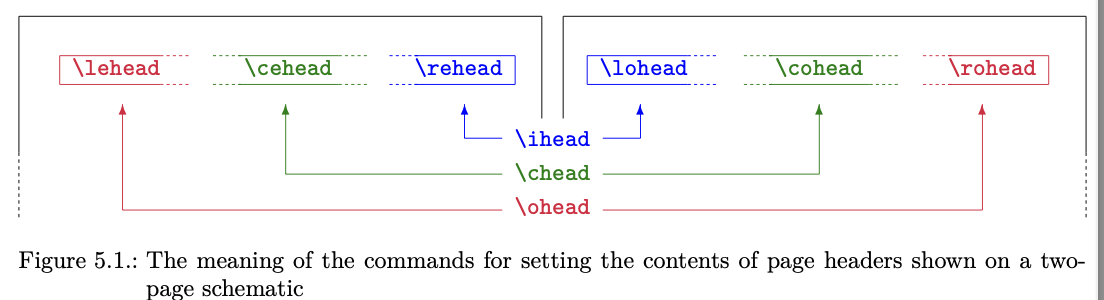
\includegraphics[width=1\linewidth]{imagem04.png}
\end{figure}

Mas o que acontece? Na primeira página, há apenas um número de página no rodapé, enquanto o cabeçalho permanece vazio!

A explicação é simples: a classe scrartcl, como a classe de artigo padrão, muda para o estilo de página simples para a página que contém o título. Após o comando \cmd{pa\-ge\-sty\-le{scr\-head\-ings}} no preâmbulo do nosso exemplo, isso realmente se refere ao estilo de página plain.scrheadings. O padrão para este estilo de página ao usar uma classe \KOMAScript\ é um cabeçalho de página vazio e um número de página no rodapé. No exemplo, os argumentos opcionais de \cmd{lohead} e \cmd{rohead} são omitidos, então o estilo de página plain.scrheadings permanece inalterado e o resultado para a primeira página está realmente correto.

O uso explícito de \cmd{pa\-ge\-sty\-le{scr\-head\-ings}} nem é necessário. O pacote já executa este comando ao carregar, então ele define automaticamente o estilo de página para scrheadings. Isso também muda não apenas os títulos de estilo de página automaticamente para scrheadings, mas também plain para plain.scrheadings.

Agora adicione texto suficiente ao exemplo após \cmd{maketitle} para que uma segunda página seja impressa. Você pode simplesmente adicionar \cmd{use\-pa\-cka\-ge\{lip\-sum\}} ao preâmbulo do documento e \cmd{lipsum} abaixo de \cmd{maketitle}. Você verá que o cabeçalho da segunda página agora contém o autor e o título do documento como queríamos.

Para comparação, você também deve adicionar o argumento opcional para 
\cmd{lohead} e \cmd{rohead}. Altere o exemplo da seguinte forma:

\begin{verbatim}
\documentclass{scrartcl}
\usepackage{scrlayer-scrpage}
\lohead[John Doe]
{John Doe}
\rohead[Page style with \KOMAScript]
{Page style with \KOMAScript}
\begin{document}
\title{Page styles with \KOMAScript}
\author{John Doe}
\maketitle
\end{document}
\end{verbatim}

Agora você tem um cabeçalho na primeira página logo acima do próprio título. Isso porque você reconfigurou o estilo de página plain.scrheadings com os dois argumentos opcionais. Como você provavelmente sabe, seria melhor deixar esse estilo de página inalterado, pois um cabeçalho acima do título do documento é bem chato.

A propósito, como uma alternativa para configurar plain.scrheadings você poderia, se você estivesse usando uma classe \KOMAScript\ ter alterado o estilo de página para páginas que contêm cabeçalhos de título. Veja \cmd{ti\-tle\-pa\-ge\-sty\-le} na seção 3.12, página 83.
Observe que você nunca deve colocar um cabeçalho de seção ou número de seção diretamente no cabeçalho usando um desses comandos. Devido à maneira assíncrona como o TeX organiza e produz páginas, fazer isso pode facilmente resultar no número errado ou texto de cabeçalho no cabeçalho corrente. Em vez disso, você deve usar o mecanismo de marcação, idealmente em conjunto com os procedimentos explicados na próxima seção.
\begin{verbatim}
\lehead*[plain.scrheadings content ]{scrheadings content}
\cehead*[plain.scrheadings content ]{scrheadings content}
\rehead*[plain.scrheadings content ]{scrheadings content}
\lohead*[plain.scrheadings content ]{scrheadings content}
\cohead*[plain.scrheadings content ]{scrheadings content}
\rohead*[plain.scrheadings content ]{scrheadings content}
\end{verbatim}

As versões com estrela dos comandos descritos anteriormente diferem das versões comuns apenas se você omitir o argumento opcional plain.scrheadings content. Neste caso, a versão sem a estrela não altera o conteúdo de plain.scrheadings. A versão com estrela, por outro lado, usa o argumento obrigatório scrheading content para plain.scrheadings também. Então, se ambos os argumentos devem ser os mesmos, você pode simplesmente usar a versão com estrela com apenas o argumento obrigatório.

\textbf{Exemplo}: Você pode encurtar o exemplo anterior usando as versões com estrela de \cmd{lohead} e \cmd{rohead}:
\begin{verbatim}
        \documentclass{scrartcl}
        \usepackage{scrlayer-scrpage}
        \lohead*{John Doe}
        \rohead*{Estilo de página com \KOMAScript}
        \begin{document}
        \title{Page styles with \KOMAScript}
        \author{John Doe}
        \maketitle
        \end{document} 
\end{verbatim}

\begin{figure}
    \centering
    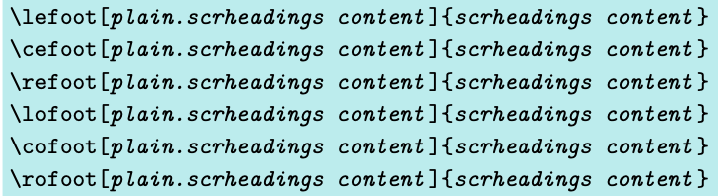
\includegraphics[width=0.8\linewidth]{imagem26.png}
\end{figure}

Você pode definir o conteúdo do rodapé para scrheadings e plain.scrheadings com estes comandos. O argumento opcional define o conteúdo de um elemento de plain.scrheadings, enquanto o argumento obrigatório define o conteúdo do elemento correspondente de scrheadings.

O conteúdo de páginas pares --- ou à esquerda --- é definido com \cmd{lefoot}, \cmd{cefoot} e \cmd{refoot}. O “e” que aparece como a segunda letra dos nomes dos comandos significa “par”.

O conteúdo de páginas ímpares --- ou à direita --- é definido com \cmd{lofoot}, \cmd{cofoot} e \cmd{rofoot}. O “o” que aparece como a segunda letra dos nomes dos comandos significa “ímpar”.

Observe que na impressão de um lado, existem apenas páginas à direita, e o \LaTeX\ as designa como páginas ímpares, independentemente do número da página.

Cada rodapé consiste em um elemento alinhado à esquerda que pode ser definido com \cmd{lefoot} ou \cmd{lofoot}. O “l” que aparece como a primeira letra dos nomes dos comandos significa “alinhado à esquerda”.

Da mesma forma, cada rodapé tem um elemento centralizado que pode ser definido com \cmd{cefoot} ou \cmd{cofoot}. O “c” na primeira letra dos nomes dos comandos significa “centralizado”.

Da mesma forma, cada rodapé tem um elemento alinhado à direita que pode ser definido com \cmd{refoot} ou \cmd{rofoot}. O “r” na primeira letra dos nomes dos comandos significa “alinhado à direita”.

No entanto, esses elementos não têm atributos de fonte individuais que podem ser alterados com os comandos \cmd{set\-ko\-ma\-font} e \cmd{add\-to\-ko\-ma\-font} (consulte a seção 3.6, página 58). Em vez disso, eles usam um elemento chamado \texttt{pa\-ge\-foot}. Antes que esse elemento seja aplicado, o elemento de fonte \texttt{pa\-ge\-head\-foot} também é aplicado. Consulte a tabela 5.1 para os padrões das fontes desses elementos.

O significado de cada comando para rodapés na impressão frente e verso é ilustrado na figura 5.2.

\textbf{Exemplo}: Vamos retornar ao exemplo do artigo curto. Digamos que você queira especificar o editor no lado esquerdo do rodapé. Você mudaria o exemplo acima para:

 \begin{verbatim}
\documentclass{scrartcl}
\usepackage{scrlayer-scrpage}
\lohead{John Doe}
\rohead{Estilo de página com \KOMAScript}
\lofoot{Smart Alec Publishing}
\usepackage{lipsum}
\begin{document}
\title{Page styles with \KOMAScript}
\author{John Doe}
\maketitle
\lipsum
\end{document}   
\end{verbatim}  

Mais uma vez, o editor não é impresso na primeira página com o título. O motivo é o mesmo do exemplo com \cmd{lohead} acima. E a solução para obter o editor na primeira página é semelhante:
\begin{verbatim}
    \lofoot[Smart Alec Publishing]{Smart Alec Publishing}
\end{verbatim}

Agora você decide que o cabeçalho e o rodapé devem usar uma fonte vertical, mas menor no lugar da fonte inclinada padrão:

\verb|\setkomafont{pageheadfoot}{\small}|

Além disso, o cabeçalho, mas não o rodapé, deve estar em negrito:

\verb|\setkomafont{pagehead}{\bfseries}|

É importante que este comando não ocorra até que scrpage-scrlayer tenha sido carregado porque a classe \KOMAScript\ define \texttt{pagehead} como um alias para \texttt{pageheadfoot}. Somente ao carregar scrpage-scrlayer o \texttt{pagehead} se tornará um elemento independente do \texttt{pageheadfoot}.

Agora adicione mais um \cmd{lipsum} e a opção \textbf{twoside} ao carregar scrartcl. Primeiro de tudo, você verá o número da página se mover do centro para a margem externa do rodapé da página, devido aos padrões alterados de scrheadings e plain.scrheadings para impressão frente e verso com uma classe \KOMAScript.

Simultaneamente, o autor, o título do documento e o editor desaparecerão da página 2. Eles só aparecem na página 3. Isso porque usamos apenas comandos para páginas ímpares. Você pode reconhecer isso pelo “o” na segunda posição dos nomes dos comandos.

\begin{figure}[h]
    \centering
    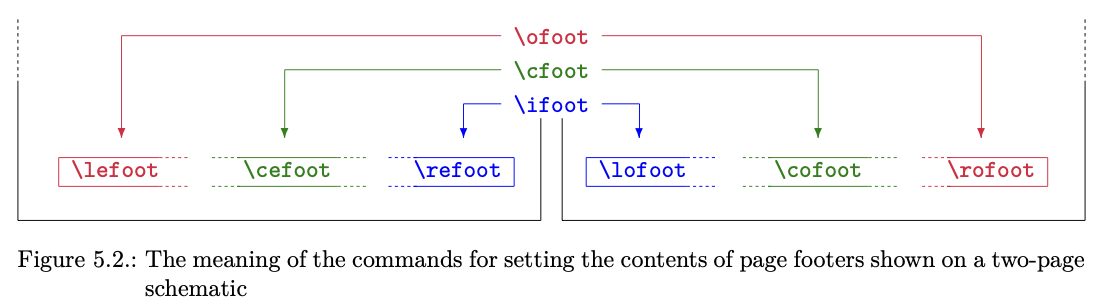
\includegraphics[width=1\linewidth]{imagem06.png}
\end{figure}

Agora, poderíamos simplesmente copiar esses comandos e substituir o “o” por um “e” para definir o conteúdo das páginas pares. Mas com a impressão frente e verso, faz mais sentido usar elementos invertidos em espelho, ou seja, o elemento esquerdo de uma página par deve se tornar o elemento direito da página ímpar e vice-versa. Para conseguir isso, também substituímos a primeira letra “l” por “r”:
\begin{verbatim}
\documentclass[twoside]{scrartcl}
\usepackage{scrlayer-scrpage}
\lohead{John Doe}
\rohead{Estilo de página com \KOMAScript}
\lofoot[Smart Alec Publishing]
{Smart Alec Publishing}
\rehead{John Doe}
\lohead{Estilo de página com \KOMAScript}
\refoot[Smart Alec Publishing]
{Smart Alec Publishing}
\usepackage{lipsum}
\begin{document}
\title{Estilos de página com \KOMAScript}
\author{John Doe}
\maketitle
\lipsum\lipsum
\end{document}
\end{verbatim}

Como é um pouco complicado definir páginas esquerda e direita separadamente em casos como o exemplo anterior, uma solução mais simples para esse caso comum é apresentada abaixo.

Permita-me mais uma vez uma observação importante: você nunca deve colocar um título de seção ou número de seção diretamente no rodapé usando um desses comandos. Devido à maneira assíncrona que o \TeX\ organiza e produz páginas, fazer isso pode facilmente resultar no número ou texto de título errado no cabeçalho corrente. Em vez disso, você deve usar o mecanismo de marcação, idealmente em conjunção com os procedimentos explicados na próxima seção.
\begin{verbatim}
\lefoot*[plain.scrheadings content ]{scrheadings content}
\cefoot*[plain.scrheadings content ]{scrheadings content}
\refoot*[plain.scrheadings content ]{scrheadings content}
\lofoot*[plain.scrheadings content ]{scrheadings content}
\cofoot*[plain.scrheadings content ]{scrheadings content}
\rofoot*[plain.scrheadings content ]{scrheadings content}  
\end{verbatim}

As versões com estrela dos comandos descritos anteriormente diferem apenas se você omitir o argumento opcional [plain.scrheadings content]. Nesse caso, a versão sem a estrela não altera o conteúdo de plain.scrheadings. A versão com estrela, por outro lado, usa o argumento obrigatório scrheading content para plain.scrheadings também.

Então, se ambos os argumentos forem iguais, você pode simplesmente usar a versão com asterisco apenas com o argumento obrigatório.

\textbf{Exemplo}: Você pode encurtar o exemplo anterior usando as versões em estrela de \cmd{lofoot} e \cmd{refoot}:
\begin{verbatim}
\documentclass[twoside]{scrartcl}
\usepackage{scrlayer-scrpage}
\lohead{John Doe}
\rohead{Estilo de página com \KOMAScript}
\lofoot*{Smart Alec Publishing}
\rehead{John Doe}
\lohead{Estilo de página com \KOMAScript}
\refoot*{Smart Alec Publishing}
\usepackage{lipsum}
\begin{document}
\title{Estilos de página com \KOMAScript}
\author{John Doe}
\maketitle
\lipsum\lipsum
\end{document} 
\end{verbatim}

\begin{verbatim}
\ohead[plain.scrheadings content ]{scrheadings content}
\chead[plain.scrheadings content ]{scrheadings content}
\ihead[plain.scrheadings content ]{scrheadings content}
\ofoot[plain.scrheadings content ]{scrheadings content}
\cfoot[plain.scrheadings content ]{scrheadings content}
\ifoot[plain.scrheadings content ]{scrheadings content} 
\end{verbatim}

Para configurar os cabeçalhos e rodapés para impressão frente e verso com os comandos descritos anteriormente, você teria que configurar os lados esquerdo e direito separadamente um do outro. Na maioria dos casos, no entanto, os lados esquerdo e direito são mais ou menos simétricos. Um item que aparece à esquerda de uma página par deve aparecer à direita de uma página ímpar e vice-versa. Elementos centralizados geralmente são centralizados em ambos os lados.

Para simplificar a definição de tais estilos de página simétricos, scrlayer-scrpage tem atalhos. O comando \cmd{ohead} corresponde a uma chamada para \cmd{lehead} e \cmd{rohead}. O comando \cmd{chead} corresponde a uma chamada para \cmd{cehead} e \cmd{cohead}. E o comando \cmd{ihead} corresponde a uma chamada para \cmd{rehead} e \cmd{lohead}. O mesmo se aplica aos comandos equivalentes para o rodapé da página. Um esboço desses relacionamentos também pode ser encontrado na figura 5.1 na página 262 e figura 5.2 na página 265.
Exemplo: Você pode simplificar o exemplo anterior usando os novos comandos:
\begin{verbatim}
\documentclass[twoside]{scrartcl}
\usepackage{scrlayer-scrpage}
\ihead{John Doe}
\ohead{Page style with \KOMAScript}
\ifoot[Smart Alec Publishing]
{Smart Alec Publishing}
\usepackage{lipsum}
\begin{document}
\title{Page styles with \KOMAScript}
\author{John Doe}
\maketitle
\lipsum\lipsum
\end{document}    
\end{verbatim}

Como a impressão unilateral trata todas as páginas como páginas ímpares, esses comandos são sinônimos dos comandos correspondentes do lado direito quando no modo unilateral. Portanto, na maioria dos casos você precisará apenas desses seis comandos em vez dos doze descritos antes.

Permita-me mais uma vez uma observação importante: você nunca deve colocar um título de seção ou número de seção diretamente no rodapé usando um desses comandos. Devido à maneira assíncrona com que o TeX organiza e produz páginas, isso pode facilmente resultar no número ou texto de título errado no cabeçalho. Em vez disso, você deve usar o mecanismo de marcação, idealmente em conjunção com os procedimentos explicados na próxima seção.
\begin{verbatim}
\ohead*[plain.scrheadings content ]{scrheadings content}
\chead*[plain.scrheadings content ]{scrheadings content}
\ihead*[plain.scrheadings content ]{scrheadings content}
\ofoot*[plain.scrheadings content ]{scrheadings content}
\cfoot*[plain.scrheadings content ]{scrheadings content}
\ifoot*[plain.scrheadings content ]{scrheadings content}
\end{verbatim}

Os comandos descritos anteriormente também têm versões com asterisco que diferem apenas se você omitir o argumento opcional [\texttt{plain.scrheadings content}]. Nesse caso, a versão sem asterisco não altera o conteúdo de \texttt{plain.scrheadings}. A versão com asterisco, por outro lado, também usa o argumento obrigatório \texttt{scrheadings content} para \texttt{plain.scrheadings}. Então se ambos os argumentos devem ser os mesmos, você pode simplesmente usar a versão com estrela com apenas o argumento obrigatório.

\textbf{Exemplo}: Você pode encurtar o exemplo anterior usando a versão com estrela de \cmd{ifoot}:
\begin{verbatim}
\documentclass[twoside]{scrartcl}
\usepackage{scrlayer-scrpage}
\ihead{John Doe}
\ohead{Estilo de página com \KOMAScript}
\ifoot*{Smart Alec Publishing}
\usepackage{lipsum}
\begin{document}
\title{Page styles with \KOMAScript}
\author{John Doe}
\maketitle
\lipsum\lipsum
\end{document} 
\end{verbatim}

\minisec{pagestyleset=setting}
Os exemplos acima se referem várias vezes às configurações padrão dos estilos de página \texttt{scrheadings} e \texttt{plain.scrheadings}. Na verdade, scrlayer-scrpage atualmente fornece dois padrões diferentes para esses estilos de página. Você pode selecioná-los manualmente com a opção \texttt{pagestyleset}.

A configuração \KOMAScript\ seleciona os padrões, que também são definidos automaticamente se a opção não for especificada e uma classe \KOMAScript\ for detectada. Na impressão frente e verso, \texttt{scrheadings} usa cabeçalhos de corrida alinhados externamente no cabeçalho e números de página alinhados externamente no rodapé. Na impressão unilateral, o cabeçalho de corrida será impresso no meio do cabeçalho e o número da página no meio do rodapé. Letras maiúsculas e minúsculas são usadas nos cabeçalhos de corrida automáticos como eles realmente aparecem nos títulos de seccionamento. Isso corresponde à opção \texttt{markcase=used}. O estilo de página \texttt{plain.scrheadings} não tem cabeçalhos correntes, mas os números de página são impressos da mesma maneira.

No entanto, se a classe \textbf{scrlttr2} for detectada, as configurações padrão serão baseadas nos estilos de página daquela classe. Veja a seção 4.13, página 230.

A configuração padrão seleciona padrões que correspondem aos estilos de página das classes padrão. Isso também é ativado automaticamente se a opção não tiver sido especificada e nenhuma classe \KOMAScript\ for detectada. Neste caso, para impressão frente e verso \texttt{scrheadings} usa cabeçalhos correntes alinhados internamente no cabeçalho, e os números de página serão impressos --- também no cabeçalho --- alinhados externamente. A impressão unilateral usa as mesmas configurações, mas como apenas páginas à direita existem neste modo, o cabeçalho corrente sempre será alinhado à esquerda e o número da página alinhado à direita. Os cabeçalhos correntes automáticos --- apesar das objeções tipográficas consideráveis --- são convertidos para letras maiúsculas, como seriam com \texttt{markcase=upper}. Na impressão de um lado, o estilo de página plain.scrheadings difere consideravelmente de \texttt{scrheadings} porque o número da página é impresso no meio do rodapé. Ao contrário do estilo de página simples nas classes padrão, \texttt{plain.scrheadings} omite o número da página na impressão frente e verso. As classes padrão imprimem o número da página no meio do rodapé, o que não corresponde ao resto dos estilos de página na impressão frente e verso. O cabeçalho é omitido em \texttt{plain.scrheadings}.

Observe que usar esta opção ativa o estilo de página \texttt{scrheadings}.



\chapter{Manipulando Estilos de Página}
Seção 5.4 explica como os estilos de páginas \texttt{scrheadings} e \texttt{plain.scrheadings} são definidos e como esses padrões podem ser alterados. Mas tópicos como criar cabeçalhos em execução, alterar as larguras do cabeçalho e rodapé e colocar linhas horizontais acima ou abaixo do cabeçalho ou rodapé ainda precisam ser descritos. Embora esses recursos sejam realmente parte do pacote \textbf{scrlayer}, eles serão explicados abaixo porque esses recursos básicos do \textbf{scrlayer} constituem uma parte importante do \textbf{scrlayer-scrpage}.

\begin{figure}[h]
    \centering
    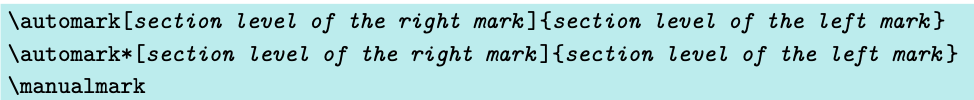
\includegraphics[width=0.9\linewidth]{imagem05.png}
\end{figure}

Tanto nas classes \LaTeX\ padrão quanto nas classes \KOMAScript\ a decisão de usar cabeçalhos automáticos ou estáticos é feita usando o estilo de página apropriado. Cabeçalhos repetem algum texto descritivo, como um título, que é apropriado para a página ou coluna, geralmente no cabeçalho, mais raramente no rodapé. Como já explicado na seção 3.12, você obtém cabeçalhos automáticos com títulos 

Nas classes de artigo \textbf{article} ou \textbf{scrartcl}, o estilo de página de títulos usa o título da seção, que é o argumento obrigatório ou opcional de \cmd{section}, para o título de documentos de um lado. Documentos de dois lados usam este título de seção como a marca esquerda e o título de subseção como a marca direita. A marca esquerda é impressa, como o nome indica, nas páginas esquerdas (verso). A marca direita é impressa nas páginas direitas (reto) — na impressão de um lado, isso significa em todas — as páginas. As classes, por padrão, também excluem a marca direita sempre que colocam o título da seção na marca esquerda.

As classes de relatório e livro começam um nível acima. Assim, elas usam o título do capítulo como a marca direita na impressão de um lado. Na impressão frente e verso, o título do capítulo é a marca esquerda e o título da seção é a marca direita.

Se você usar \texttt{myheadings}, as marcas no cabeçalho da página ainda existirão, e os números de página serão colocados da mesma forma, mas os comandos de seção não definem mais as marcas automaticamente. Você pode defini-las manualmente usando os comandos \cmd{markright} e \cmd{markboth}, que são descritos mais adiante nesta seção.

Essa distinção foi eliminada pelo \textbf{scrlayer}. Em vez de distinguir entre cabeçalhos automáticos e manuais pelo estilo de página selecionado, há dois novos comandos:
\begin{verbatim}
    \automark
    \manualmark
\end{verbatim}

O comando \cmd{manualmark} alterna para marcas manuais e desativa o preenchimento automático das marcas. Em contraste, \cmd{automark} e \cmd{automark*} definem quais níveis de seção devem ser usados para definir a marca automaticamente. O argumento opcional é o nível de seção da marca direita, o argumento obrigatório é o nível de seção da marca esquerda. Os argumentos devem sempre ser o nome de um nível de seção como parte, capítulo, seção, subseção, subsubseção, parágrafo ou subparágrafo.

Normalmente, o nível mais alto deve ser usado para a marca esquerda e o nível mais baixo para a marca direita. Isso é apenas uma convenção e não um requisito, mas faz sentido.

Observe que nem toda classe fornece cabeçalhos de execução para cada nível de seção. Por exemplo, as classes padrão nunca usam \cmd{part} no título. As classes \KOMAScript\ por outro lado, suportam todos os níveis.

A diferença entre \cmd{automark} e \cmd{automark*} é que \cmd{automark} substitui todos os comandos anteriores para definir automaticamente a marca, enquanto \cmd{automark*} altera apenas o comportamento dos níveis de seção especificados em seus argumentos.

\textbf{Exemplo}: Suponha que você queira que os títulos dos capítulos sejam usados como cabeçalho de páginas pares e o título da seção seja o cabeçalho de páginas ímpares, como de costume. Mas em páginas ímpares você também quer que os títulos dos capítulos sejam usados como cabeçalho até que a primeira seção apareça. Para fazer isso, primeiro você precisa carregar o \textbf{scrlayer-scrpage} e selecionar o estilo de página \texttt{scrheadings}, para que o documento comece com:
\begin{verbatim}
\documentclass{scrbook}
\usepackage{scrlayer-scrpage}
\pagestyle{scrheadings} 
\end{verbatim}

Em seguida, certifique-se de que os títulos dos capítulos definam as marcas da esquerda e da direita: \cmd{automark[chapter]\{chapter\}}

Então o título da seção também deve definir as marcas da direita:

\verb|\automark*[section]{}|

Aqui, a versão com estrela é usada, já que o comando \cmd{automark} anterior deve permanecer em vigor. Além disso, o argumento obrigatório para o nível de seção da marca da esquerda está vazio porque essa marca deve permanecer inalterada.

Tudo o que falta agora é um pouco de conteúdo do documento para mostrar o resultado:
\begin{verbatim}
\usepackage{lipsum}
\begin{document}
\chapter{Título do Capítulo}
\lipsum[1-20]
\section{Título da Seção}
\lipsum[21-40]
\end{document}  
\end{verbatim}

Usamos o pacote extremamente útil \textit{lipsum} para gerar algum texto fictício com comando \cmd{lipsum}.

Se você testar o exemplo, verá que a primeira página do capítulo aparece, como de costume, sem um título corrente, já que esta página usa automaticamente o estilo de página simples \texttt{plain.scrheadings} (ver sobre \cmd{chap\-ter\-pa\-ge\-sty\-le} na página 83). As páginas 2–4 têm os títulos dos capítulos no título corrente. Após o título da seção na página 4, o título corrente da página 5 muda para este título da seção. Desta página até o final, o título corrente alterna de página para página entre os títulos do capítulo e da seção.

\begin{figure}[h]
    \centering
    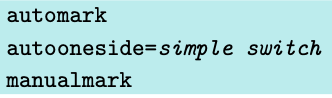
\includegraphics[width=0.5\linewidth]{imagem07.png}
\end{figure}

Em vez dos comandos descritos anteriormente, você também pode usar as opções \texttt{manualmark} e \texttt{automark} para alternar entre cabeçalhos de execução automáticos e manuais. \texttt{automark} sempre usa o padrão \cmd{automark[section]\{chapter\}} para classes com \cmd{chapter} e \cmd{automark[subsection]\{section}\} para outras classes.

Na impressão unilateral, você normalmente quer que apenas os níveis de seção mais altos forneçam o título de execução. A opção padrão \texttt{autooneside} corresponde a esse comportamento. A opção aceita os valores para interruptores simples listados na tabela 2.5, página 41. Se você desativar essa opção, os argumentos opcionais e obrigatórios de \texttt{automark} e \texttt{automark*} controlarão novamente o cabeçalho de execução na impressão unilateral.

\textbf{Exemplo}: Suponha que você tenha um relatório unilateral, mas queira títulos semelhantes aos do exemplo de livro anterior. Especificamente, os títulos dos capítulos devem ser usados como título até que a primeira seção apareça. Daí em diante, o título da seção deve ser usado. Então, modificamos um pouco o exemplo anterior:
\begin{verbatim}
\documentclass{scrreprt}
\usepackage[autooneside=false]{scrlayer-scrpage}
\pagestyle{scrheadings}
\automark[section]{chapter}
\usepackage{lipsum}
\begin{document}
\chapter{Título do capítulo}
\lipsum[1-20]
\section{Título da seção}
\lipsum[21-40]
\end{document}    
\end{verbatim}

Como você pode ver, um comando \texttt{automark*} não é necessário neste caso. Você deve tentar o exemplo com \texttt{autooneside} definido como \textit{true} ou remover a opção para comparação. Você notará uma diferença no cabeçalho de execução da página 4 em diante.
Note que apenas carregar o pacote não tem efeito algum sobre se cabeçalhos de execução automáticos ou manuais são usados, ou que tipo de cabeçalhos de seccionamento preenchem as marcas. Somente usando explicitamente a opção \texttt{automark} ou \texttt{manualmark}, ou o comando \cmd{automark} ou \cmd{manualmark}, as condições aqui serão inicializadas.

\begin{figure}[h]
     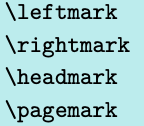
\includegraphics[width=0.2\linewidth]{imagem08.png}
\end{figure}

Se você quiser se afastar dos estilos de página predefinidos, normalmente precisa decidir onde colocar o conteúdo das marcas. Com \cmd{left\-mark} você pode definir o que aparecerá na marca esquerda quando a página for impressa.

Da mesma forma, você pode usar \cmd{right\-mark} para definir o conteúdo da marca direita.

Você pode facilitar a vida com \cmd{headmark}. Esta extensão do \textbf{scrlayer} é uma abreviação que resolve para \cmd{left\-mark} ou \cmd{right\-mark} dependendo se a página atual é par ou ímpar.

O comando \cmd{pagemark} não tem nada a ver com o mecanismo de marca do TeX. Ele é usado para exibir um número de página formatado. A fonte do elemento \texttt{pagenumber} será usada para a saída. Isso pode ser alterado usando os comandos \cmd{set\-ko\-ma\-font} ou \cmd{add\-to\-ko\-ma\-font} (veja também a seção 3.6, página 58).

\textbf{Exemplo}: Suponha que você queira que o cabeçalho seja alinhado à margem esquerda e o número da página à margem direita na impressão unilateral. O seguinte exemplo mínimo de trabalho faz exatamente isso:
\begin{verbatim}
\documentclass{scrreprt}
\usepackage{blindtext}
\usepackage[automark]{scrlayer-scrpage}
\pagestyle{scrheadings}
\ihead{\headmark}
\ohead*{\pagemark}
\chead{}
\cfoot[]{}
\begin{document}
\blinddocument
\end{document}  
\end{verbatim}

O pacote \texttt{blindtext} e seu comando \cmd{blind\-do\-cu\-ment} foram usados aqui para gerar rapidamente o conteúdo do documento de amostra para o exemplo.

Os comandos \cmd{ihead} e \cmd{ohead*} configuram as marcas desejadas. A variante \cmd{ohead*} com estrela também configura o número da página com o estilo de página \texttt{plain.scrheadings} usado na primeira página de um capítulo.

Como esses estilos de página têm marcas predefinidas no centro do cabeçalho e rodapé, esses elementos são limpos usando \cmd{chead} e \cmd{cfoot} com argumentos vazios. Como alternativa, você pode usar \cmd{clear\-pair\-of\-pa\-ge\-sty\-les} antes de \cmd{ihead}. Você encontrará esse comando descrito na seção 18.2.

Observe que o argumento opcional vazio de \cmd{cfoot} no exemplo acima não é o mesmo que omitir o argumento opcional. Você deve tentar você mesmo e dar uma olhada na diferença no rodapé da primeira página.

Usuários avançados podem encontrar mais comandos de configuração de marca a partir da página 448.

\begin{figure}[h]
    \centering
    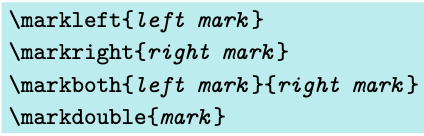
\includegraphics[width=0.5\linewidth]{imagem09.png}
\end{figure}

Independentemente de você estar trabalhando com cabeçalhos de execução manuais ou automáticos, você pode sempre alterar o conteúdo da marca esquerda ou da marca direita usando esses comandos. Observe que a marca à esquerda resultante de \cmd{leftmark} será a última marca colocada na página correspondente, enquanto a marca à direita resultante de \cmd{rightmark} é a primeira marca colocada na página correspondente. Para mais detalhes, consulte \cmd{ri\-ght\-first\-mark} na seção 17.6, página 443.

Se você estiver usando cabeçalhos de execução manuais, as marcas permanecerão válidas até que sejam explicitamente substituídas pela reutilização dos comandos correspondentes. No entanto, se você estiver usando cabeçalhos de execução automáticos, as marcas podem se tornar inválidas com o próximo título de seção, dependendo da configuração automática.

Você também pode usar esses comandos em conjunto com as versões com estrela dos comandos de seção.

\textbf{Exemplo}: Suponha que você escreva um prefácio de várias páginas colocadas logo antes do índice mas não aparecendo nele. No entanto, como você usa linhas divisórias no seu cabeçalho, você quer um cabeçalho para este prefácio:
\begin{verbatim}
\documentclass[headsepline]{book}
\usepackage{scrlayer-scrpage}
\pagestyle{scrheadings}
\usepackage{blindtext}
\begin{document}
\chapter*{Preface}
\markboth{Preface}{Preface}
\blindtext[20]
\tableofcontents
\blinddocument
\end{document}    
\end{verbatim}

À primeira vista, isso parece produzir o resultado desejado. Dando uma segunda olhada, no entanto, você pode ver que o título “Preface” não aparece em letras maiúsculas, ao contrário dos outros cabeçalhos. Mas isso é fácil de mudar:
\begin{verbatim}
\documentclass[headsepline]{book}
\usepackage{scrlayer-scrpage}
\pagestyle{scrheadings}
\usepackage{blindtext}
\begin{document}
\chapter*{Preface}
\markboth{\MakeMarkcase{Preface}}{\MakeMarkcase{Preface}}
\blindtext[20]
\tableofcontents
\blinddocument
\end{document}   
\end{verbatim}

Usar o comando \cmd{MakeMarkcase} resulta na obtenção da mesma caixa de letras que para cabeçalhos de execução automáticos.

Agora, vamos mover o \cmd{tableofcontents} para a frente do prefácio e remover o comando \cmd{markboth}. Você descobrirá que o prefácio agora tem o cabeçalho de execução “CONTENTS”. Isso se deve a uma peculiaridade do \cmd{chapter*} (veja também a seção 3.16 na página 105).

Se você não quiser um cabeçalho de execução aqui, você pode facilmente fazer isso passando dois argumentos vazios para \cmd{markboth}:
\begin{verbatim}
\documentclass[headsepline]{book}
\usepackage{scrlayer-scrpage}
\pagestyle{scrheadings}
\usepackage{blindtext}
\begin{document}
\tableofcontents
\chapter*{Preface}
\markboth{}{}
\blindtext[20]
\blinddocument
\end{document}    
\end{verbatim}

O comando \cmd{markdouble} altera a marca esquerda e a marca direita para o mesmo conteúdo. Então \cmd{mark\-dou\-ble\{mark\}} é uma forma mais curta de \cmd{mark\-both\{mark\}\-\{mark\}} com dois argumentos idênticos.


% \include{chap23}
% \include{chap24}



\backmatter
\chapter{Dicta}
Um elemento comum em um documento é uma epígrafe ou citação que é definida acima ou abaixo de um título de capítulo ou seção, junto com uma referência à fonte e sua própria formatação. \KOMAScript\ se refere a tal epígrafe como um dictum.
\begin{verbatim}
    \dictum[Schiller]{So pause ye who would link your fates~\dots}}
\end{verbatim}





\end{document}
